\documentclass{lincolncsuthesis}

% Packages you want to use
% Packages you intend to use
% ..

% For example, if you want to render 
% the document in a different font you can
% use something like: 

%\usepackage{gentium}
%\usepackage{txfonts}
%\usepackage[sfdefault]{roboto}


% Or maybe you want clickable references in your thesis:
\usepackage{url}
\usepackage{hyperref}
\usepackage{biblatex}
\usepackage[UKenglish]{babel}
\usepackage[T1]{fontenc}
\usepackage[utf8]{inputenc}
\usepackage{lmodern}
\usepackage{paralist}
\usepackage{fancyhdr}
\usepackage{amsmath, amssymb, amsfonts}
\usepackage{mathtools}
\usepackage{framed}
\usepackage{pstricks}
\usepackage[amsmath,framed, thmmarks, standard]{ntheorem}
\usepackage[usenames,dvipsnames,svgnames,table]{xcolor}
\usepackage[backref=true,                % 
            hyperref=true,               % 
            firstinits=true,             %
            indexing=true,               %
            url=false,                   % 
            style=ieee,            %  style=debug, alphabetic
            backend=biber,               % 
            doi=false,
            texencoding=utf8,
            bibencoding=utf8]{biblatex}

% Bibliography setup: import bib files
% Add in the .bib files you wish to add 
% into your document here. If you want to
% include others, just copy this line and
% change the path!

\addbibresource{./bib/references.bib}


% This thesis template also supports rendering
% a ludography. To cite games, make sure your reference
% in your bib file has keywords={game} in the bibtex item.
%
% See the bib file below for an example.

% \addbibresource{bib/ludography.bib}

% Your thesis details -- edit the file at the path below
% so it shows your name, title, etc. 
%% Below are a bunch of details for formatting your undergraduate thesis.
%% Make sure to fill each of these out.

% The title of your thesis (If your title is very large, consider prepending
% it with the \Large command
\title{\bfseries SLAM Implementation and Benchmarking}

% Your name, as an author
\author{Mangal Deep.B.M}

% The degree
\thesisDegree{M.Eng}

% The programme
\thesisProgramme{Embedded Systems for Mechatronics}

% The school name
\thesisSchool{School of Informatics}

% The university you're studying at (Lincoln!)
% The university (UoL)
\thesisUniversity{Dortmund University of Applied Sciences and Arts}

% Your student number
\thesisStudentNumber{7206937}

% The date (which is shown last, you can just put a year in here):
\date{15-3-2021}



% What will be displayed in the header: the assessment item
\thesisHeaderContents{Research Thesis}

% Uncommenting the \thesisTurnOffHF line below will remove your name + id from the footer
% as well as removing the header contents. It is NOT recommended to do this
% as the presentation policy for assessed work in the SoCS requires
% these both of these. However, you may want to uncomment this for other
% reasons: i.e. when printing a personal copy which is NOT going to be
% submitted.
% -----
% \thesisTurnOffHF
% -----
\title{SLAM - Implementation and Benchmarking}
\author{Mangal Deep .B.M}

\begin{document}

% First, make the title
\maketitle{}

% Input anything that can go before the acknowledgements 
% The blank page environment allows you to insert
% pages into your thesis for specific things

\begin{blankpage}
    \chapterTitle{A blank page}
    This is an optional page environment you could use for things like:
	\begin{itemize}
		\item Your own custom preamble chapters (use \texttt{\textbackslash chapterTitle} for titles!)
		\item \emph{``This work is dedicated to Dad and Mom''}
		\item A copyright notice
		\item Additional notes
		\item Quotes
		\item List of publications
		\item An actual blank page
		\item Nomenclature / glossaries, etc.
	\end{itemize}
	It is not recommended to use this in your undergraduate thesis for submission. It has been left in here to make you aware of its existence. This is largely because it does not follow the guidelines set out for undergraduate theses, but you could include this environment for your own personal printed copy. Consult with your supervisor to see if you can use it. 
	
	In addition, you can pass an optional parameter to this environment with the value \texttt{c} to centre this text vertically on the page (use the \texttt{center} environment to align horizontally).
\end{blankpage}


% Then the abstract
\begin{abstract}
    This is where your abstract will go. Usually this is written last, after writing the entirety of your thesis.
\end{abstract}

% Then the acknowledgements
\begin{acknowledgements}
Firstly, I want to thank somebody, and somebody else.\footnote{Here is a footnote} Here is another note.
\end{acknowledgements}

% Print out the table of tables and table of figures and
% tell the template we're about to start the body of the
% thesis.
\thesisTables
% Indexes, Glossaries

\thesisBodyStart
% start of thesis body
% ---------------------------

% Include introduction
\chapter{Introduction}
Accurate determination of relative poses is a key element in many robotic applications. \textit{Scan-Matching} is the method of registering two scans from perception sensors taken from two poses to determine the relative transformation between the two poses. It is the key step in successfully and efficiently solving \textit{Simultaneous Localization and Mapping} problem. The pose information available to the robot in motion are erroneous and mapping with such information can result in inaccurate map of the environment.Various scan matching algorithms are widely used in many applications that are uniquely developed for a particular type of perception sensor. Generally, It corrects the pose information obtained from the motion sensors with the information obtained from the perception sensors\cite{GMap_algo}. With the advent of new sensors and improvement to the existing sensors, it is also possible to solve the \textit{Simultaneous Localization and Mapping} problem only with perception sensors \cite{loam}.

\textit{Simultaneous Localization and Mapping}, commonly abbreviated as \textit{SLAM} is one of the fundamental and essential task of any mobile robots that builds map of the environment without the knowledge of actual location and orientation of the robot. It is one of the key initial step for the development of navigation systems for any mobile robot. It is also referred as  the chicken or the egg problem, as it requires precise location of the robot in the environment, to get an accurate map of the environment, but in order to determine the precise location, the map of the environment is required. Given the complexity it is  harder to find a precise solution, accurate localization and mapping.

The complex task of localizing and mapping the surrounding has triggered a huge interest widely in the research filed and it continues to  improve as the technology evolves in both software and hardware. Over the past decade numerous strategies and methods \cite{A.Pratik}, \cite{E.Olson_Map}, \cite{T.seb_survey}, \cite{D.Hahnel}, \cite{M.Montemerlo}, \cite{W.Burgard}, \cite{GMap_algo}, \cite{G.Grisetti}, \cite{J.Kang}, \cite{K.Konolige}, \cite{W.Burgard}, \cite{T.Reineking}, \cite{D.Droeschel}, \cite{SUMA++}, \cite{VPS_SLAM}, \cite{RT_Graph}, \cite{chen2020rss}, \cite{loam}, \cite{ChanWF}, \cite{TatenoTLN17}, \cite{K.Ryu}, \cite{faucris.119665744}, \cite{Lu-2016-5572}, \cite{Mur_Artal_2015}, \cite{Mur_Artal_2017}, \cite{P.Agarwal}, \cite{segmap2018} were developed to solve the SLAM problem. 

A typical SLAM system uses a combination of odometry data, GPS, IMU to obtain information on the motion and Camera, LiDAR or Radar to observe the environment. The information obtained from these sensors are fused to obtain a full estimate of the state of the system. Though technologies evolved in acquiring precise measurement uncertainties and errors are still prevalent due to various factors. Hence designing a solution considering the uncertainties in the measurement is a key to achieve a good estimate of the location and map of the surrounding. Therefore a probabilistic approach is the key to globally consistent map.

The SLAM problem can be classified in various ways.SLAM problem can be broadly classified into \textit{Online SLAM} and \textit{Full SLAM}. In the \textit{Online SLAM} problem, only the current state of the robot is estimated along with the map. In the \textit{Full SLAM} problem, the entire state of the path traversed by the robot is estimated.Based on the environment to be mapped, the SLAM system can be broadly classified into \textit{Feature-based SLAM} and \textit{Grid-based SLAM}. In \textit{Feature-based SLAM}, the robot looks for specific features or landmarks in the surrounding, the map obtained from it will specify the shape of the environment only at the landmark locations. However in real world scenarios, the robot should establish a correspondence between the expected landmark measurement and the actual landmark observed. The data association plays a key role in assigning the measurement to  its corresponding landmarks. With the known correspondence and known pose of the robot relative to a landmark, the problem reduces to Mapping with known pose. The \textit{Feature-based SLAM} is widely applied in many robotics application for instance, underwater exploration\cite{6678293}, mapping underground mines. These SLAM systems commonly use Ultrasonic sensors, camera for perception and GPS, odometry are used to find the motion of the robot.

In absence of landmarks, \textit{Grid-based SLAM} provides a complete SLAM solution with the help of 2-D or 3-D laser scanners or cameras. The observations made by the LiDAR are converted to an obstacle map also referred to as occupancy map. These observations are also used to correct the pose estimate of the robot. This SLAM approach provides a more useful way to map the surroundings as landmarks cannot be installed and observed in many challenging environment. Common approaches to \textit{Grid-based SLAM} are \textit{Particle Filters} and \textit{Graph Networks} More details on this approach will be provided in the chapter 4.

Numerous research has been done in the SLAM community. Some of the implementations are made available to the public in \textit{Robotic Operating system (ROS)} framework,commonly abbreviated as \textit{ROS}. The most common are \textit{gMapping}\cite{gmap_ros} and \textit{Cartographer}\cite{cartographer_ros}.

This thesis presents insights on different scan-matching methods by applying it to Particle Filter based SLAM algorithm, namely \textit{gMapping}. These algorithms are implemented, tested and results are compared thoroughly to provide detailed report on throughput of the algorithms. The algorithm is tested on the data set obtained from \textit{CARLA}\cite{Dosovitskiy17}.\textit{CARLA} is an open-source simulator for autonomous driving research and development. It provides the environment for algorithm development, validation and testing. For more information on \textit{CARLA}, refer to \cite{Dosovitskiy17}. In this work  \textit{CARLA} is used extensively to gather data, that is also used to implement various scan-matching algorithm and compare its performance .In the \textit{CARLA} simulator, an autonomous driving car mounted with sensors such as LiDAR, GNSS and IMU is driven through the simulated environment and all required data are collected in ROSBag through the ROS Bridge that establishes communication between  \textit{ROS} framework and \textit{CARLA}. The LiDAR is the perception system in the simulated car. It is a 360 degrees 3D LiDAR with 32 beams with a range of 50 meters rotating at a  frequency of 20 Hertz. The aforementioned sensors are placed at the same geometrical position on the vehicle and are oriented in the same direction that is also aligned to the vehicle coordinate system. The ISO sign convention is used for all the coordianted frames throughout this work and the convention defines  \textit{x}-axis(longitudinal axis) is pointing forward,  \textit{y}-axis (lateral axis) pointing left,  \textit{z}-axis (normal)pointing upward and the rotation is positive in the counter-clockwise direction. This avoids transforming measurements to different coordinate systems. The system is developed for an autonomous driving car trying to create a 2D map of the simulated environment. Hence from this point, map generally refers to grid map, pose refers to Special Euclidean (SE2) and orientation, unless specified. 

 The thesis is organized as follows: The detailed literature review is provided on existing scan-matching methods, SLAM algorithms and applications, variants of SLAM in chapter \ref{chap:Literature}. Probabilistic formulation of the scan-matching and SLAM problem is derived in chapter \ref{chap:Formulation}. Particle Filter based solution to SLAM is discussed and different implementations such as Rao-Blackwellized Particle Filter and gMapping algorithm are discussed in detail and analyzed in chapter \ref{chap:Particle}. Scan-matching methods are discussed in detail in chapter \ref{chap:Scan}. Comparison and bench-marking of the scan-matching methods are performed based on test results and computation is provided in chapter \ref{chap:Comparison}. Concluding remark on all the observations made so far in the paper is discussed in chapter \ref{chap:Conclusions}.

% Literature review / Background / Related work
\chapter{Literature review}
% General Literature introduction
    The state of a robot such as position, orientation, velocity, acceleration, parameters or even a map, is critical to get accurate results. 
    Needless to mention, the more information the robot knows about itself, the solution to find unknowns becomes easier. 
    In the context of SLAM, pose information and the map of the environment are the states of absolute interest. 
    Given the high precision pose information of the robot, then the problem simplifies to mapping of the environment with known pose.Here the state of interest is 
    only the map which does not even require state estimation rather use the available mapping algorithm to draw the Map of the environment. 
    On the other hand, given the Map of the environment, then the problem reduces to localization problem with data association in certain cases. 
    Here the state of interest is pose and the correspondence for data association. A survey on various \textit{SLAM} methods were presented by 
    \cite{C.Cadena} and \cite{T.Takleh}. According to \cite{C.Cadena}, the history of SLAM is broadly classified into \textit{classical age} 
    consisting of \textit{Extended Kalman Filter (EKF)} methods, \textit{Rao-Blackwellized Particle Filter (RBPF)} methods and \textit{Maximum Likelihood Estimation}. 
    Followed by \textit{algorithmic-analysis age} which predominantly studied observability, convergence and consistency of SLAM, 
    leading to efficient SLAM solvers and many open source libraries. Followed by \textit{robust-perception age} which focuses on robust performance, 
    Resource awareness, high level understanding and task-driven perception.Finally in my perspective, with the development and up-rise in the application of 
    Deep Learning techniques in SLAM, it would be suitable to term the current trend as \textit{Machine Learning era of SLAM}

% SLAM - Kalman Filter based
    In the beginning, hardware capabilities were very less and compute power embedded in mobile robots were limited to fewer processes at an instance. Hence the choice of sensors to be mounted on 
    the robots were very critical. Historically the very first feasible solution to the SLAM problem proposed the use of Extended Kalman Filters(EKFs) by estimating the joint posterior distribution 
    over pose of the robot and the landmark positions.Kalman Filters are widely used state estimators but are limited to linear system and works on the assumption of Gaussian distribution of data.
    Therefore they cannot be directly applied to solve the non-linear SLAM problems. By linearizing the data at the mean of the distribution it is possible to approximate the solution, the Extended
    Kalman Filter works on this principle. The state estimate and the associated uncertainty are provided by the mean and covariance matrix of the posterior of the joint probability. 
    However the odometric drift observed by the robot seems to hold down the accuracy of the posterior estimate.\cite{J.Kang} proposed  modified 
    Neural Network aided EKF (mNNEKF) to improve the accuracy of the estimate by compensating for odometric error of the robot using Neural Network. This method claims to work well even under
    colored noise and systematic bias error.
% SLAM - Particle Filter based


% SM - ICP
% SLAM - Graph Network based

% SLAM - Neural Network based

% SLAM - conclusion


%%%%%%%%%%%%%%%%%%%%%%%%%%%%%%%%%%%%%%%%%%%%%%%%%%%%%%%%%%%%%%%%%%%%%%%%%%%%%%%%%%%%%%%%%%%%%%%
% Another cool thing about \LaTeX~is its referencing system. This template is set up to use harvard-style referencing. You can do this by using \texttt{\textbackslash citep\{citekey\}}. It will print out something like this: \citep{aad2012observation}. Or alternatively, you can use \texttt{\textbackslash cite\{citekey\}} to cite things like this: \cite{chatrchyan2012observation}. This template uses Bib\LaTeX~for referencing, with a Biber backend. This is primarily due to the extensive features Bib\LaTeX~provides, along with the option of glossaries. If you want to customise the referencing style, you can either modify the template slightly to use different options, or use \texttt{\textbackslash usepackage} again to reimport it. There's probably some commands to change its options after its been imported too.

% \section{Ludography}
% This thesis template also contains an optional ludography. This is primarily for Games Development students, who wish to cite games in their thesis. To use this, just put references into your bib file as usual with the game's details. Then, make sure \texttt{keywords} is set to \texttt{\{game\}}. This is what is used to determine which references are games, and which are actual papers. For a more elaborate example, see \texttt{bib/ludography.bib}.

% Also, make sure that the \texttt{title} key is actually the author of the game, and the \texttt{author} is the title of the game. The reason this is swapped around is because Bib\LaTeX~likes to print references out with the author first. Then, just add \texttt{\textbackslash printLudography} with an optional title argument to print out all citations like \texttt{\textbackslash printLudography} or \texttt{\textbackslash printLudography[Games]}.

% You can also use the \texttt{ludography} environment if you wish to print out some text before the list of games is printed. An example of this can be seen in \texttt{main.tex}. To cite games, you can \texttt{\textbackslash cite} it like any other reference. However, if you want it to display the title instead of the standard referencing style, you can use \texttt{\textbackslash citeGame} instead.

% Here is an example of a cited game with a normal reference style: ~\cite{spaceinvaders}. Ugh, pretty ugly. Instead, here the two are  cited in the next sentence as games with \texttt{\textbackslash citeGame}. Both \citeGame{spaceinvaders} and \citeGame{breakout} were games made by Atari. Much better!

% SLAM Formulation + State Prediction and correction
\chapter{Formulation}
\section{Introduction}

%%%%%%%%%%%%%%%%%%%%%%%%%%%%%%%%%%%%%%%%%%%%%%%%%%%%%%%%%%%%%%%%%%%%%%%%%%%%%%%%%%%%%%%%%%%%%%%%%%%%%%%%%%%%%%
\section{Probabilistic approach to state estimation}

%%%%%%%%%%%%%%%%%%%%%%%%%%%%%%%%%%%%%%%%%%%%%%%%%%%%%%%%%%%%%%%%%%%%%%%%%%%%%%%%%%%%%%%%%%%%%%%%%%%%%%%%%%%%%%
\section{State Prediction}
\subsection{Odometry Motion Models}
\subsection{Kinematic Motion Models}

%%%%%%%%%%%%%%%%%%%%%%%%%%%%%%%%%%%%%%%%%%%%%%%%%%%%%%%%%%%%%%%%%%%%%%%%%%%%%%%%%%%%%%%%%%%%%%%%%%%%%%%%%%%%%%
\section{State Correction}
\subsection{Observation Models}
\subsection{Scan Matching}

%%%%%%%%%%%%%%%%%%%%%%%%%%%%%%%%%%%%%%%%%%%%%%%%%%%%%%%%%%%%%%%%%%%%%%%%%%%%%%%%%%%%%%%%%%%%%%%%%%%%%%%%%%%%%%
\section{Summary}

\chapter{Particle Filter}
\section{Introduction}

%%%%%%%%%%%%%%%%%%%%%%%%%%%%%%%%%%%%%%%%%%%%%%%%%%%%%%%%%%%%%%%%%%%%%%%%%%%%%%%%%%%%%%%%%%%%%%%%%%%%%%%%%%%%%%
\section{Particle Filter}
\subsection{Sample}
\subsection{Import weighting}
\subsection{Resample}

%%%%%%%%%%%%%%%%%%%%%%%%%%%%%%%%%%%%%%%%%%%%%%%%%%%%%%%%%%%%%%%%%%%%%%%%%%%%%%%%%%%%%%%%%%%%%%%%%%%%%%%%%%%%%%
\section{Rao-Blackwellized Particle Filter}

%%%%%%%%%%%%%%%%%%%%%%%%%%%%%%%%%%%%%%%%%%%%%%%%%%%%%%%%%%%%%%%%%%%%%%%%%%%%%%%%%%%%%%%%%%%%%%%%%%%%%%%%%%%%%%
\section{gMapping-Improved RBPF}

%%%%%%%%%%%%%%%%%%%%%%%%%%%%%%%%%%%%%%%%%%%%%%%%%%%%%%%%%%%%%%%%%%%%%%%%%%%%%%%%%%%%%%%%%%%%%%%%%%%%%%%%%%%%%%
\section{Results and Analysis}

%%%%%%%%%%%%%%%%%%%%%%%%%%%%%%%%%%%%%%%%%%%%%%%%%%%%%%%%%%%%%%%%%%%%%%%%%%%%%%%%%%%%%%%%%%%%%%%%%%%%%%%%%%%%%%
\section{Summary}

\chapter{Factor  Graphs}
\input{chapters/9_graphapproach}

\chapter{Comaprison and Benchmarking}
\section*{Introduction}
    The availability of various sensor technologies, scan matching algorithms for applications like SLAM requires methods and framework to validate the algorithms in an accurate way. However validating only the scan matching algorithm would not provide sufficient justification on how effective the system is. Since this work applies scan matching algorithms to SLAM, validating the output of the whole SLAM system would provide insight on how efficient and accurate are the scan matching algorithms. \cite{kuemmerle09auro} proposed metrics on evaluating the SLAM algorithms. It provides a common performance measure for various SLAM approaches. This metric calculates the performance not based on the map but the trajectory, enabling the metric to be applied across all the map representations and sensor setup. 

\section{Evaluation metric}
Consider the car moves from a position ${x_1}$  to another ${x_t}$ in time $T$, let the error accumulated be $\epsilon$. This directly leads to the equation \ref{eq:err_metric}.
\begin{gather} \label{eq:err_metric}
    \epsilon(x_{1:T}) = \sum^T_{t=1}{(x_t \ominus x_t^*)^2}
\end{gather}
where $\ominus$ is the inverse pose composition. The equation \ref{eq:err_metric} considers only the measured pose $x$ and the true(reference) pose $x*$. However it is sub-optimal \cite{kuemmerle09auro} as generally the error is carried on until the end of the simulation, but when the generated map is shifted by the error and used for comparison then the propagated error vanishes, that provides inappropriate performance insights. 
Therefore \cite{kuemmerle09auro} proposes a metric based on relative displacement between poses. The metric is given by equation \ref{eq:err_metric_final}. 
\begin{gather} \label{eq:err_metric_final}
    \epsilon(\delta) = \frac{1}{N}\sum_{i,j}{trans(\delta_{i,j} \ominus \delta_{i,j}^*)^2 + rot(\delta_{i,j} \ominus \delta_{i,j}^*)^2}
\end{gather}
where $\delta_{i,j} = x_i \ominus x_j$ and $\delta_{i,j}^* = x_i^* \ominus x_j^*$. In the above equation absolute error can be used instead of squared error. The reference pose $x^*$ can be obtained from either GPS or using \textit{Monte-Carlo localization} technique. In this work GPS is used as a pose reference

\section{Analyzing algorithms with pre-recorded CARLA Dataset}
A scenario is recorded from the CARLA simulator using ROSBag.The simulation time in the dataset is  432 seconds. The overview of the scenario \ref{fig:Scenario} and the ground truth from GNSS and Odometry \ref{fig:GT_param} are presented. The path traversed by the car is highlighted in green on the picture and the simulated car itself in orange. The \ref{fig:GT_param} provides information on pose information in simulated world coordinates, orientation, velocity, acceleration and steering angle. The vehicle halts at several traffic junctions during the simulation, however such situations are not considered in the analysis.
    \begin{figure}[h] 
        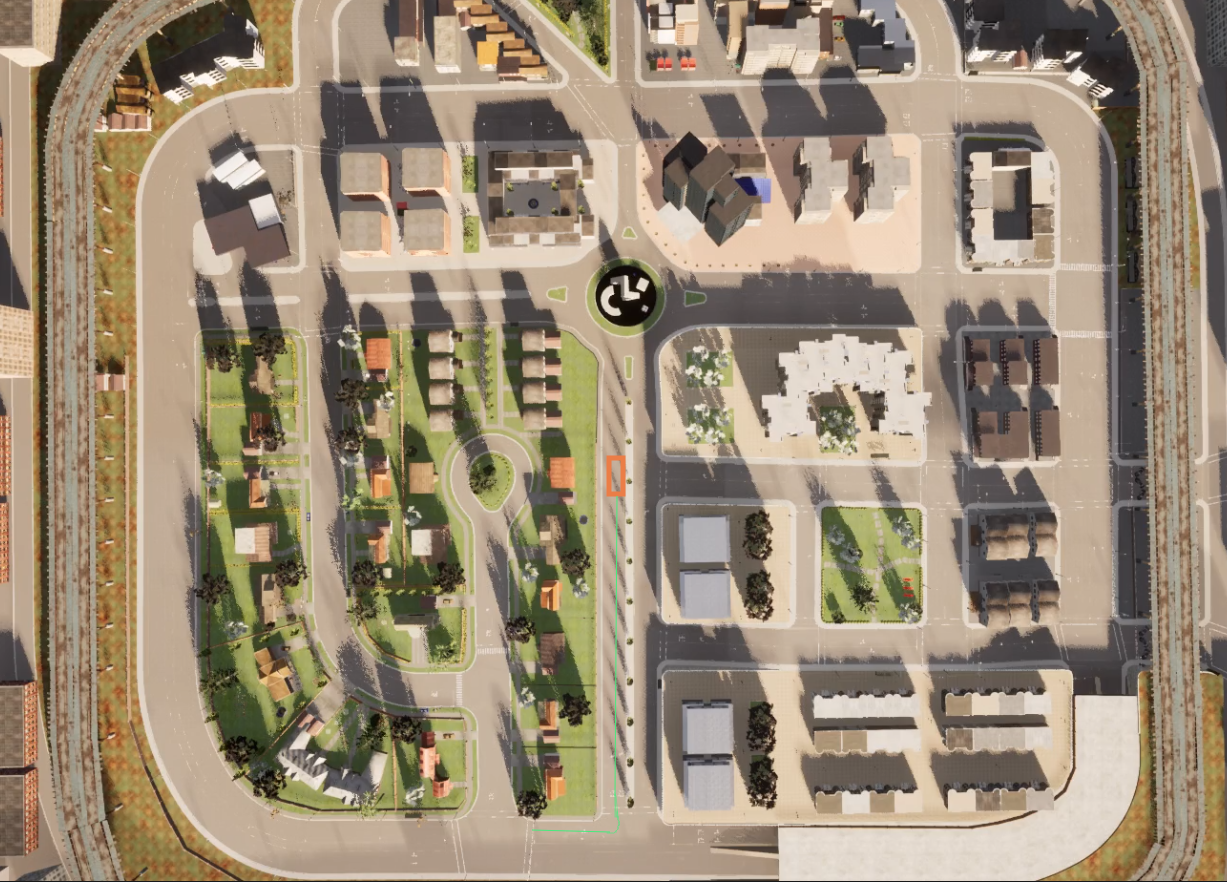
\includegraphics[height=0.6\textwidth]{images/Scenario.png}
        \caption{Scenario used in evaluation}
        \label{fig:Scenario}
    \end{figure}
    \begin{figure}[h] 
        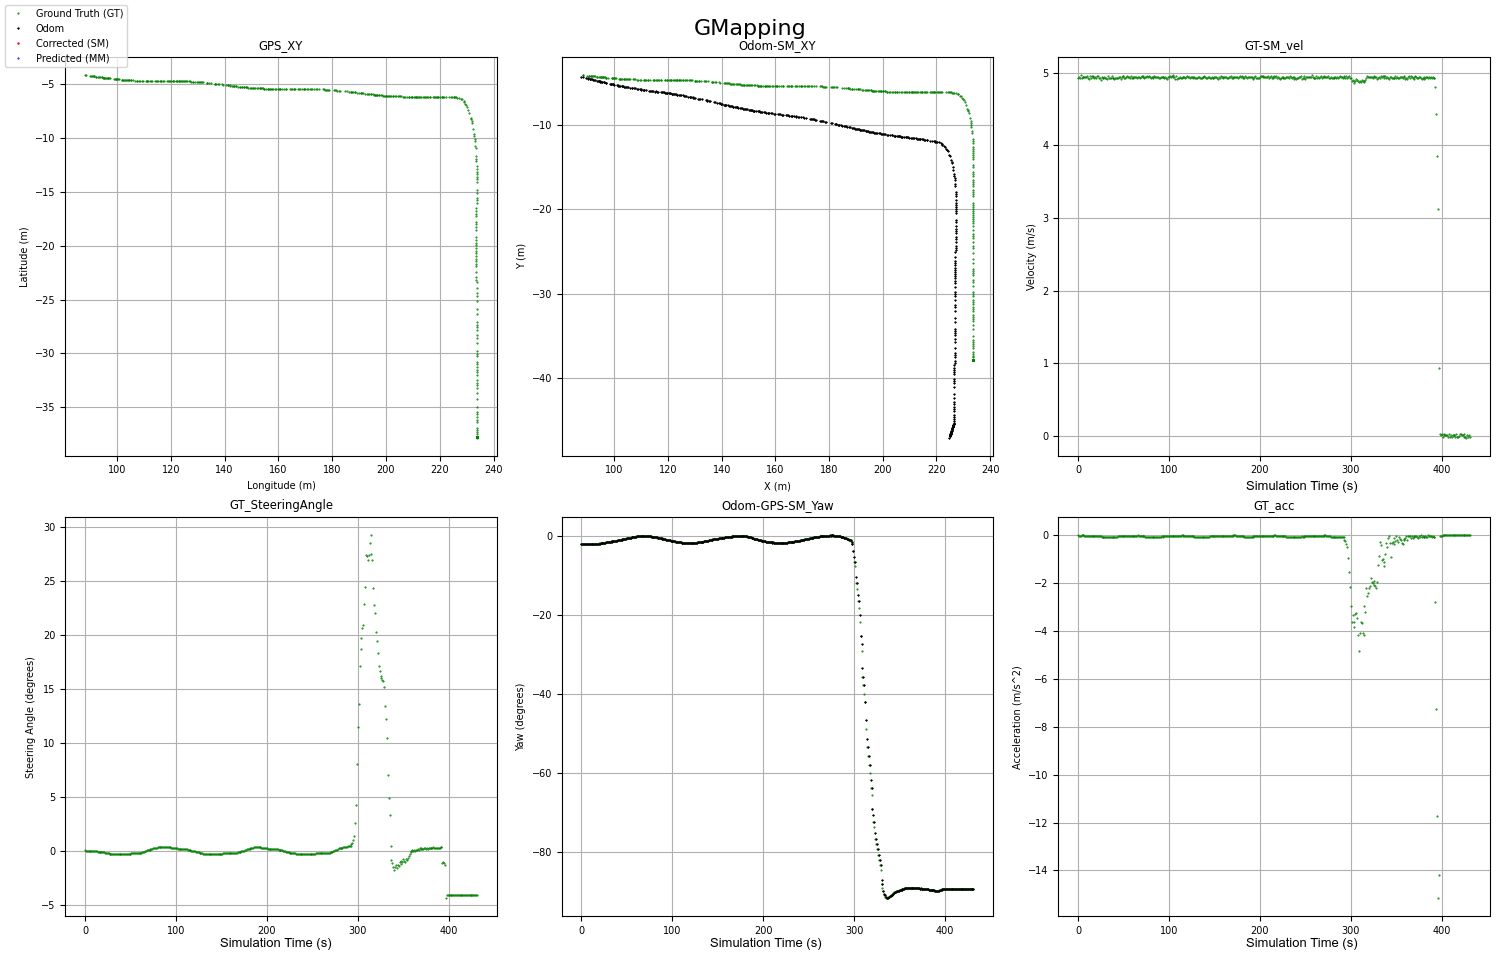
\includegraphics[height=0.6\textwidth]{images/GroundTruthParameters.png}
        \caption{Ground truth from GNSS and Odometry}
        \label{fig:GT_param}
    \end{figure}
    \begin{figure}[h] 
        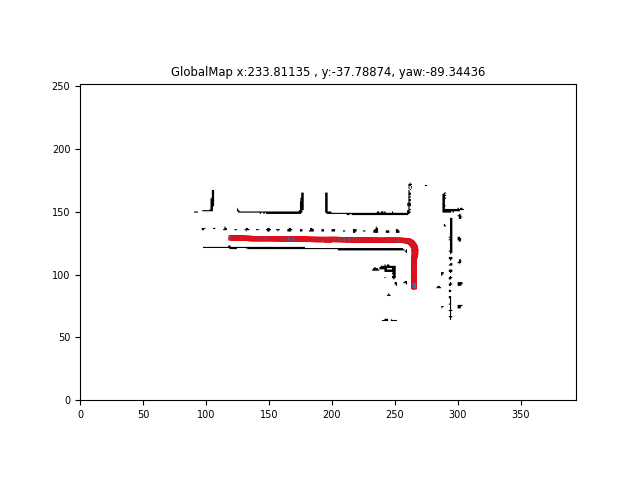
\includegraphics[height=0.6\textwidth]{images/GroundTruthMap.png}
        \caption{Map generated from GPS(ground truth)}
        \label{fig:GT_MAP}
    \end{figure}
The map generated from GPS is shown in \ref{fig:GT_MAP}
Since the odometry data from CARLA is noiseless and drift free, noise (Gaussian 0.1) and drift (modeled as a ramp function with slope 0.1) are manually added to the recorded data. The raw pose information obtained from GNSS sensor are in real coordinates in degrees, that is later converted to Cartesian coordinate system. The ground truth for the orientation is obtained from Inertial Measurement Unit (IMU). The signals velocity$(m/s)$, acceleration$(m/s^2)$ and steering angle$(degrees)$ are obtained from vehicle status message. The algorithm contains many tuning parameters that could be used for tuning and experimenting the results. However tuning parameters such as odometry noise and slope  would not be efficient as the scan matching algorithm could possibly reject its effect because of the error threshold parameter.
\clearpage
\par
LiDAR sensor mounted on the simulated car is noisy and finding the correct alignment using the scan matching algorithms usually provide results with residual error which provides confidence on how valid the results of the scan matching could be. Based on the residual error the particle filter decides if the correction step can be calculated with the scan matching results. In other words, If the scan matching error is more than a predefined threshold, the correction step is skipped and only prediction step is used to update the particle information.
Hence different thresholds of the error for scan matching algorithms discussed in the previous chapter is used in evaluating the implemented algorithms. 
\par
Finding the right correspondence between the scan points is the key to precise results in scan matching. In the implemented algorithm a constant threshold is used to assign the correspondences. Experiments were conducted with various values and different values led to instability in scan matching results. Hence this parameter is also necessary to be tuned. However this parameter variations is not considered in the analysis.
\par
In case of GMapping, the particles are used to describe the posterior density $p(x_t, m | z_{1:t}, u_{0:t-1})$. Therefore to get an accurate estimate of pose and map, the posterior density has to be calculated precisely. Intuitively with more number of particles the posterior density can be estimated accurate. Hence the number of particles is also considered as a parameter that is tuned in order to evaluate the implemented algorithms. However this has effects on the computation efficiency leading to more computational resources and time.
\par
Apart from the metrics proposed in \cite{kuemmerle09auro},Run time of the algorithms is also compared. The algorithm runs with parallel processing ensuring efficient utilisation of the compute power. The evaluation is run on a workbench equipped with AMD Ryzen 7 4800H 2,9GHz processor and 16GB RAM. The cumulative comparison is provided in \ref{ssec:overallanalysis}.

\subsection{Evaluating SVD based ICP}
The evaluation of algorithms performed with error threshold set to 0.0015 and  0.001 along with particle count 20 and 50 are presented in below figures. It can be observed that with tighter thresholds, where the erroneous scan matching results are neglected, performs better. With more number of particles the final pose values are close to ground truth GPS data.
With lenient error threshold(0.0015) and less number of particles(20), a offset can be observed in the pose and orientation estimation\ref{fig:SVD_20_0.0015}. It can also be seen that difference in the pose and orientation estimation to the ground truth is never converging \ref{fig:SVD_20_0.0015_diff}
    \begin{figure}[h] 
        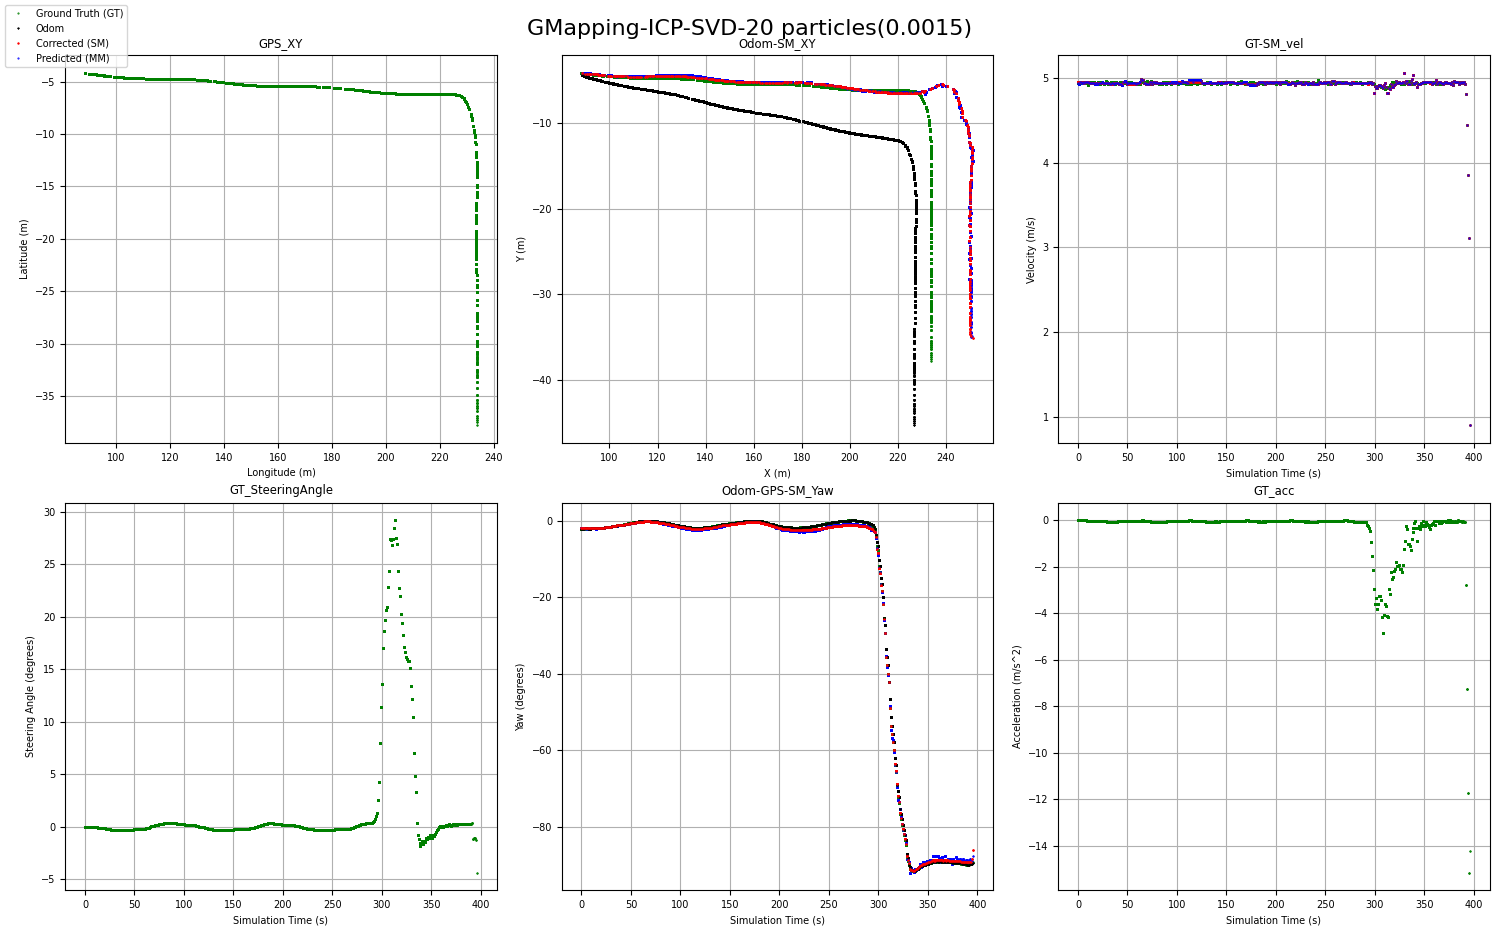
\includegraphics[height=0.6\textwidth]{images/GMapping-ICP-SVD-20 particles(0.0015)_PositionParameters.png}
        \caption{SVD based ICP- Particles(20), Error Threshold(0.0015). Label:Ground Truth(green), Odometry(black), Motion Model prediction(blue), Scan Matching correction(red)}
        \label{fig:SVD_20_0.0015}
    \end{figure}
    \begin{figure}[h] 
        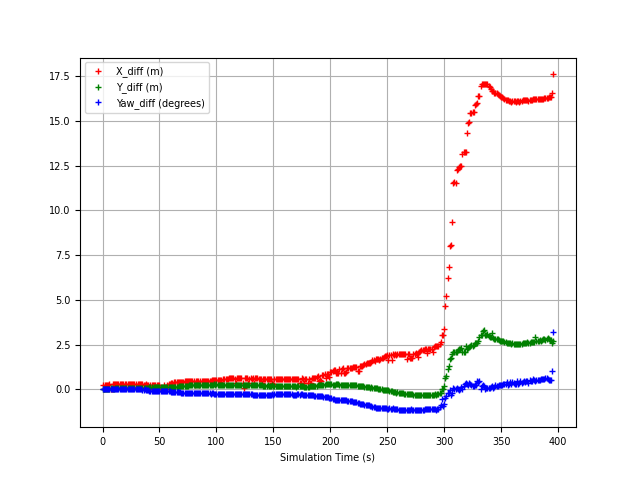
\includegraphics[height=0.4\textwidth]{images/GMapping-ICP-SVD-20 particles(0.0015)_True_vs_Crct.png}
        \caption{SVD based ICP- Difference between ground truth (GPS) and estimation}
        \label{fig:SVD_20_0.0015_diff}
    \end{figure}
\clearpage
Just increasing the number of particles to 50, provides marginally better results than the previous case \ref{fig:SVD_50_0.0015}, \ref{fig:SVD_50_0.0015_diff}
    \begin{figure}[h] 
        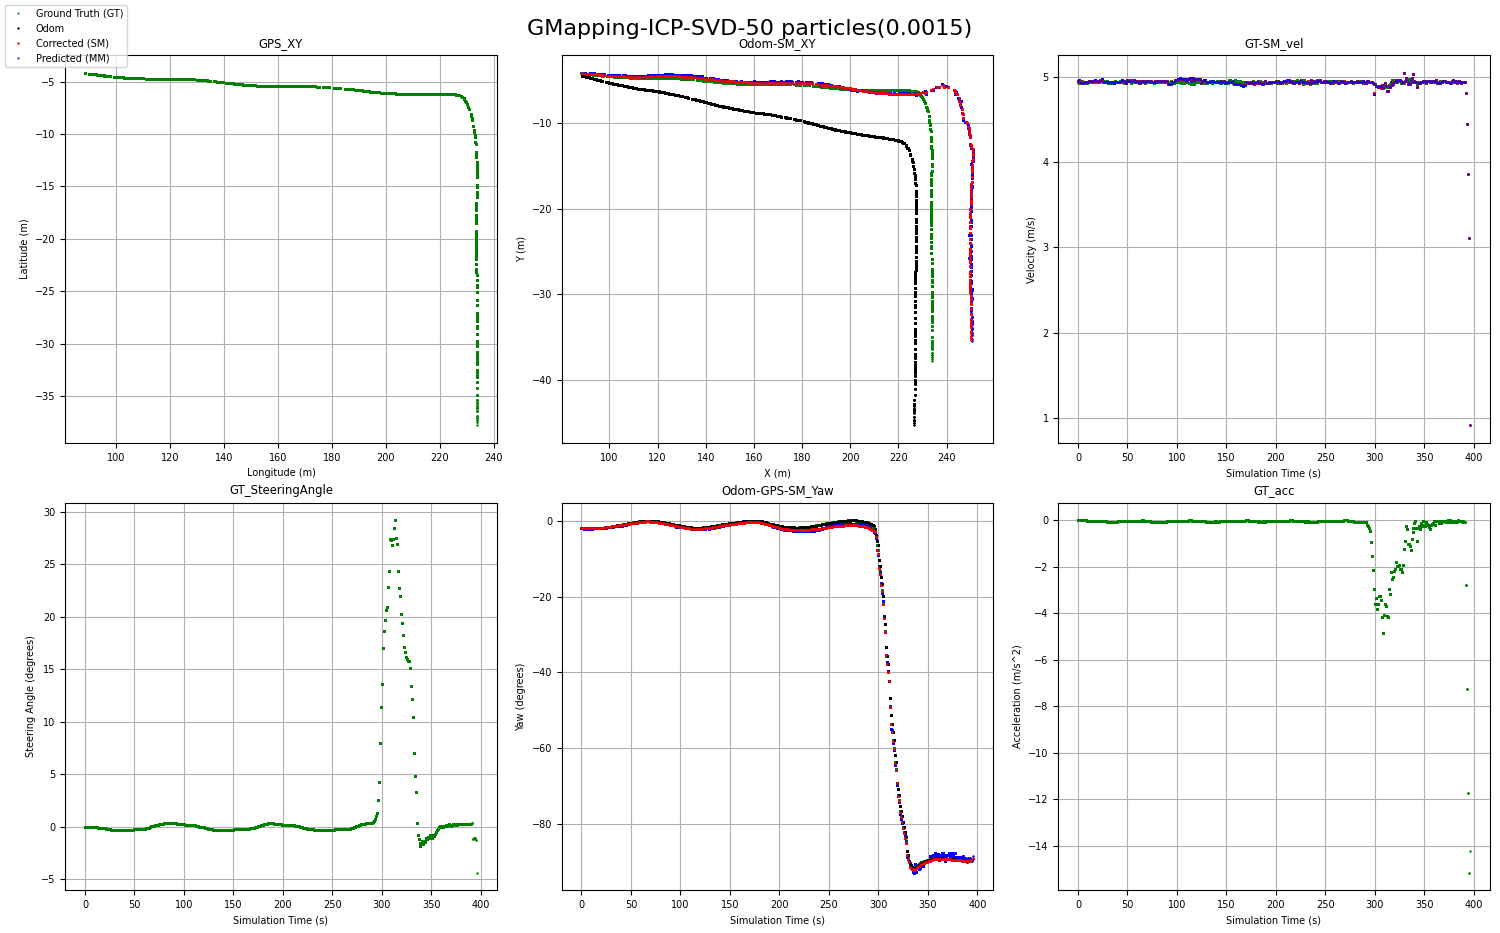
\includegraphics[height=0.6\textwidth]{images/GMapping-ICP-SVD-50 particles(0.0015)_PositionParameters.png}
        \caption{SVD based ICP- Particles(50), Error Threshold(0.0015). Label:Ground Truth(green), Odometry(black), Motion Model prediction(blue), Scan Matching correction(red)}
        \label{fig:SVD_50_0.0015}
    \end{figure}
    \begin{figure}[h]
        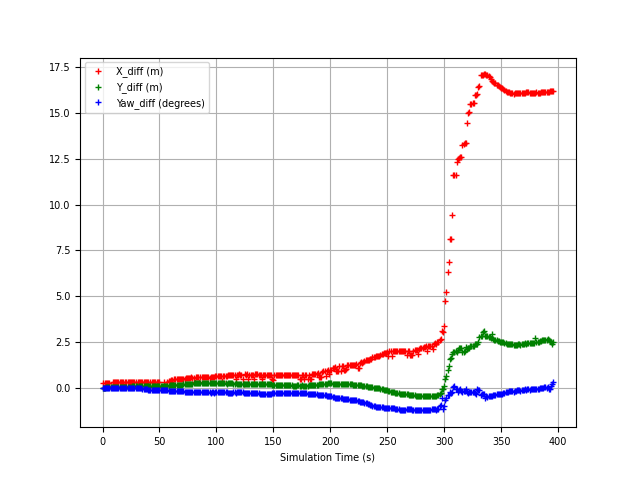
\includegraphics[height=0.4\textwidth]{images/GMapping-ICP-SVD-50 particles(0.0015)_True_vs_Crct.png}
        \caption{SVD based ICP- Difference between ground truth (GPS) and estimation}
        \label{fig:SVD_50_0.0015_diff}
    \end{figure}
\clearpage
However with tighter error threshold(0.001) the performance of the system is better, with pose more aligned to the ground truth \ref{fig:SVD_20_0.001}, \ref{fig:SVD_20_0.001_diff}.
    \begin{figure}[h] 
        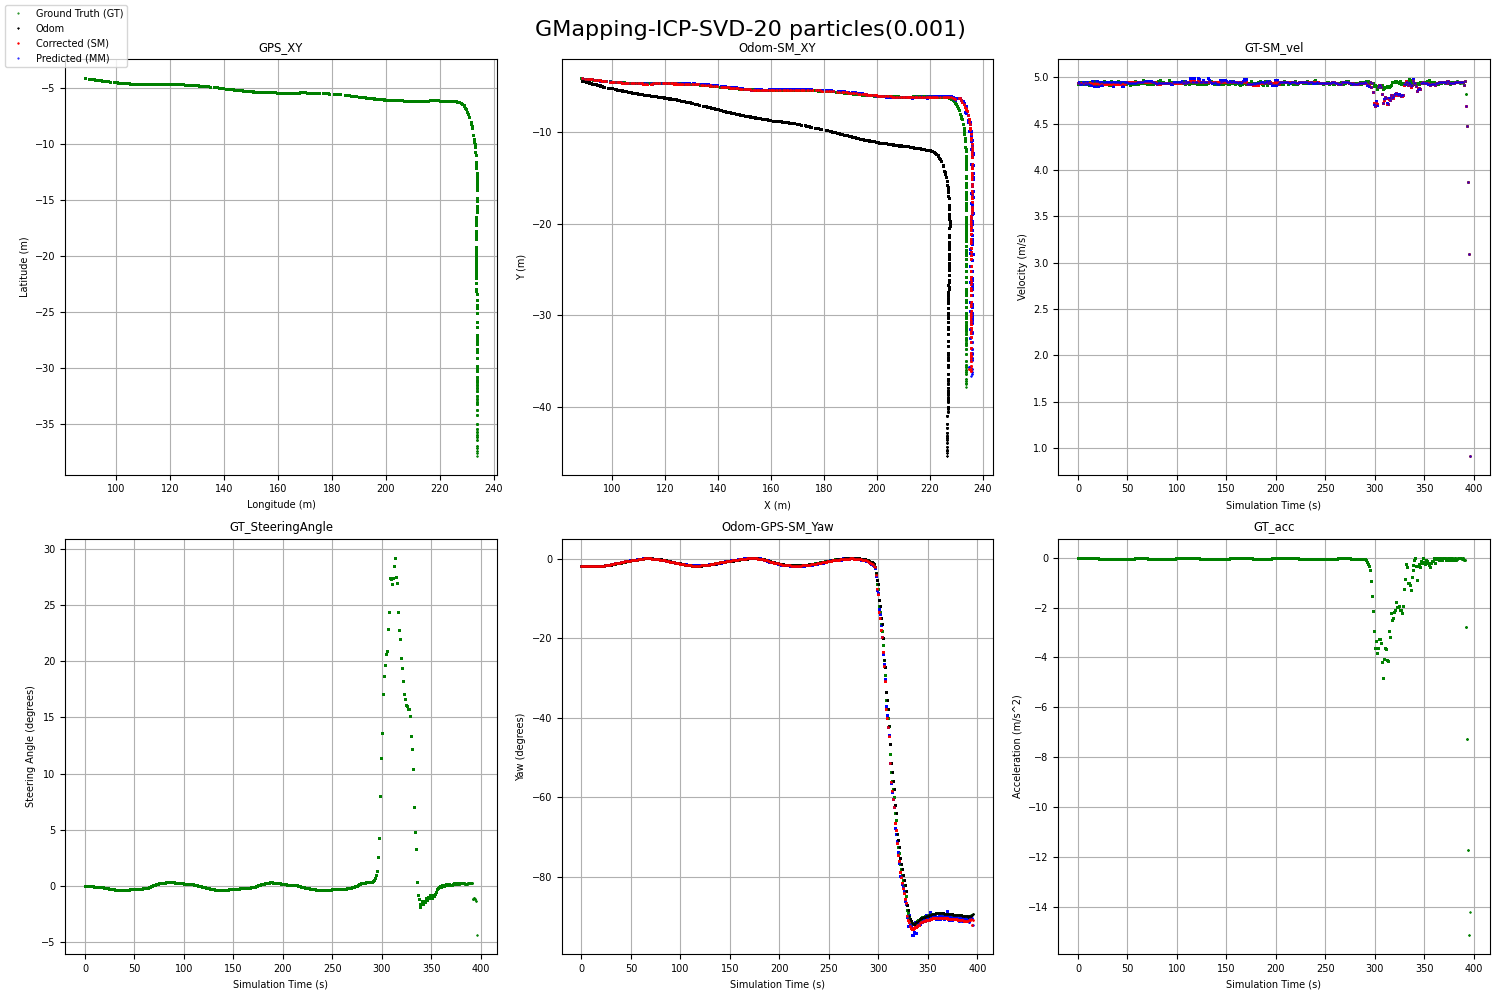
\includegraphics[height=0.6\textwidth]{images/GMapping-ICP-SVD-20 particles(0.001)_PositionParameters.png}
        \caption{SVD based ICP- Particles(20), Error Threshold(0.001). Label:Ground Truth(green), Odometry(black), Motion Model prediction(blue), Scan Matching correction(red)}
        \label{fig:SVD_20_0.001}
    \end{figure}
    \begin{figure}[h] 
        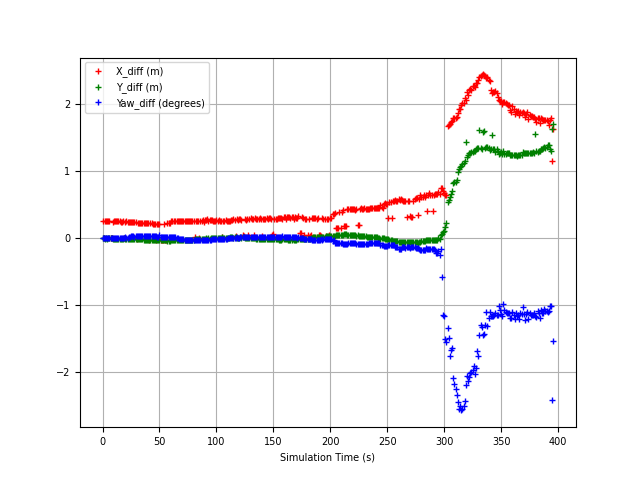
\includegraphics[height=0.4\textwidth]{images/GMapping-ICP-SVD-20 particles(0.001)_True_vs_Crct.png}
        \caption{SVD based ICP- Difference between ground truth (GPS) and estimation}
        \label{fig:SVD_20_0.001_diff}
    \end{figure}
\clearpage
With more number of particles, the results are even better \ref{fig:SVD_50_0.001}, \ref{fig:SVD_50_0.001_diff}
    \begin{figure}[h] 
        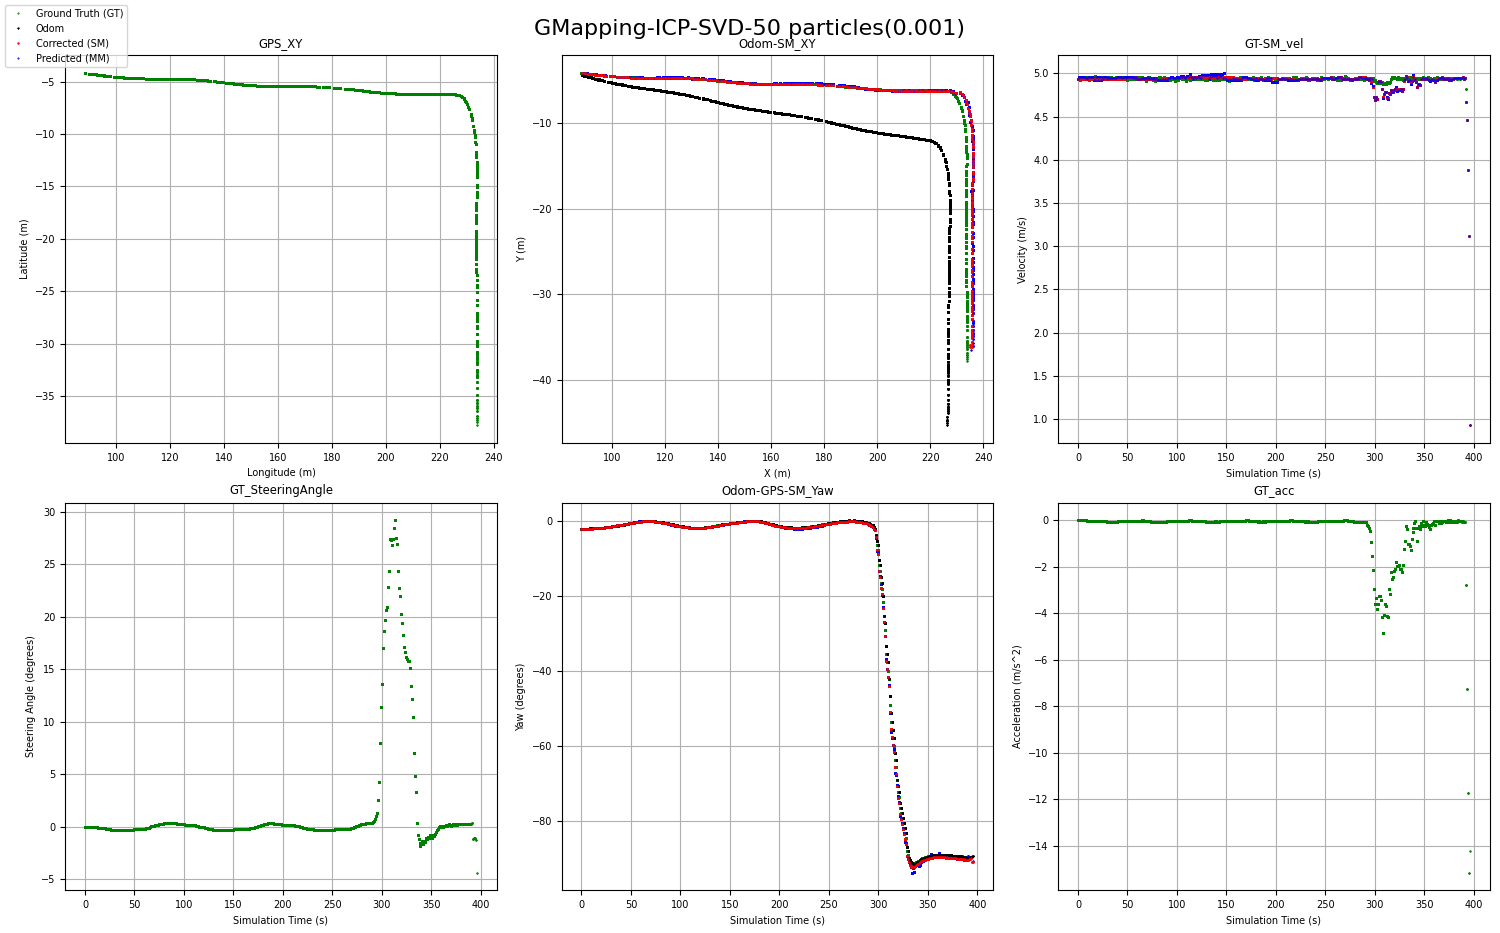
\includegraphics[height=0.6\textwidth]{images/GMapping-ICP-SVD-50 particles(0.001)_PositionParameters.png}
        \caption{SVD based ICP- Particles(50), Error Threshold(0.001). Label:Ground Truth(green), Odometry(black), Motion Model prediction(blue), Scan Matching correction(red)}
        \label{fig:SVD_50_0.001}
    \end{figure}
    \begin{figure}[h] 
        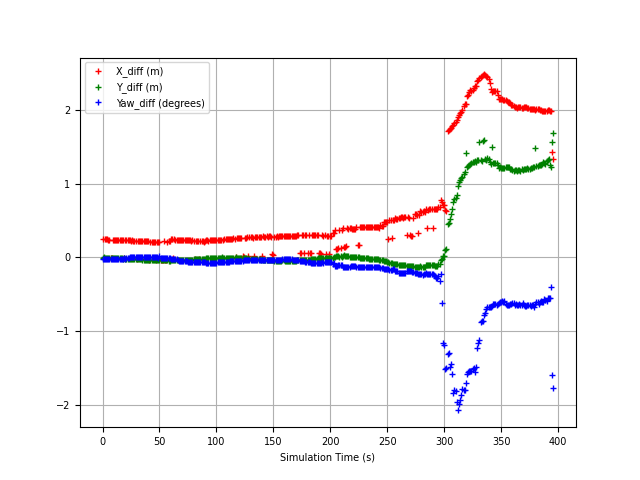
\includegraphics[height=0.4\textwidth]{images/GMapping-ICP-SVD-50 particles(0.001)_True_vs_Crct.png}
        \caption{SVD based ICP- Difference between ground truth (GPS) and estimation}
        \label{fig:SVD_50_0.001_diff}
    \end{figure}
\clearpage

\subsection{Evaluating LS based ICP}
The evaluation of algorithms performed with error threshold set to 0.0015 and  0.001 along with particle count 20 and 50 are presented in below figures. It can be observed that with tighter thresholds, where the erroneous scan matching results are neglected, performs better. With more number of particles the final pose values are close to ground truth GPS data.
With lenient error threshold(0.0015) and less number of particles(20), a offset can be observed in the pose and orientation estimation\ref{fig:LS_20_0.0025}. Like in the case of SVD based ICP, It can also be seen that difference in the pose and orientation estimation to the ground truth is never converging \ref{fig:LS_20_0.0025_diff}.
    \begin{figure}[h] 
        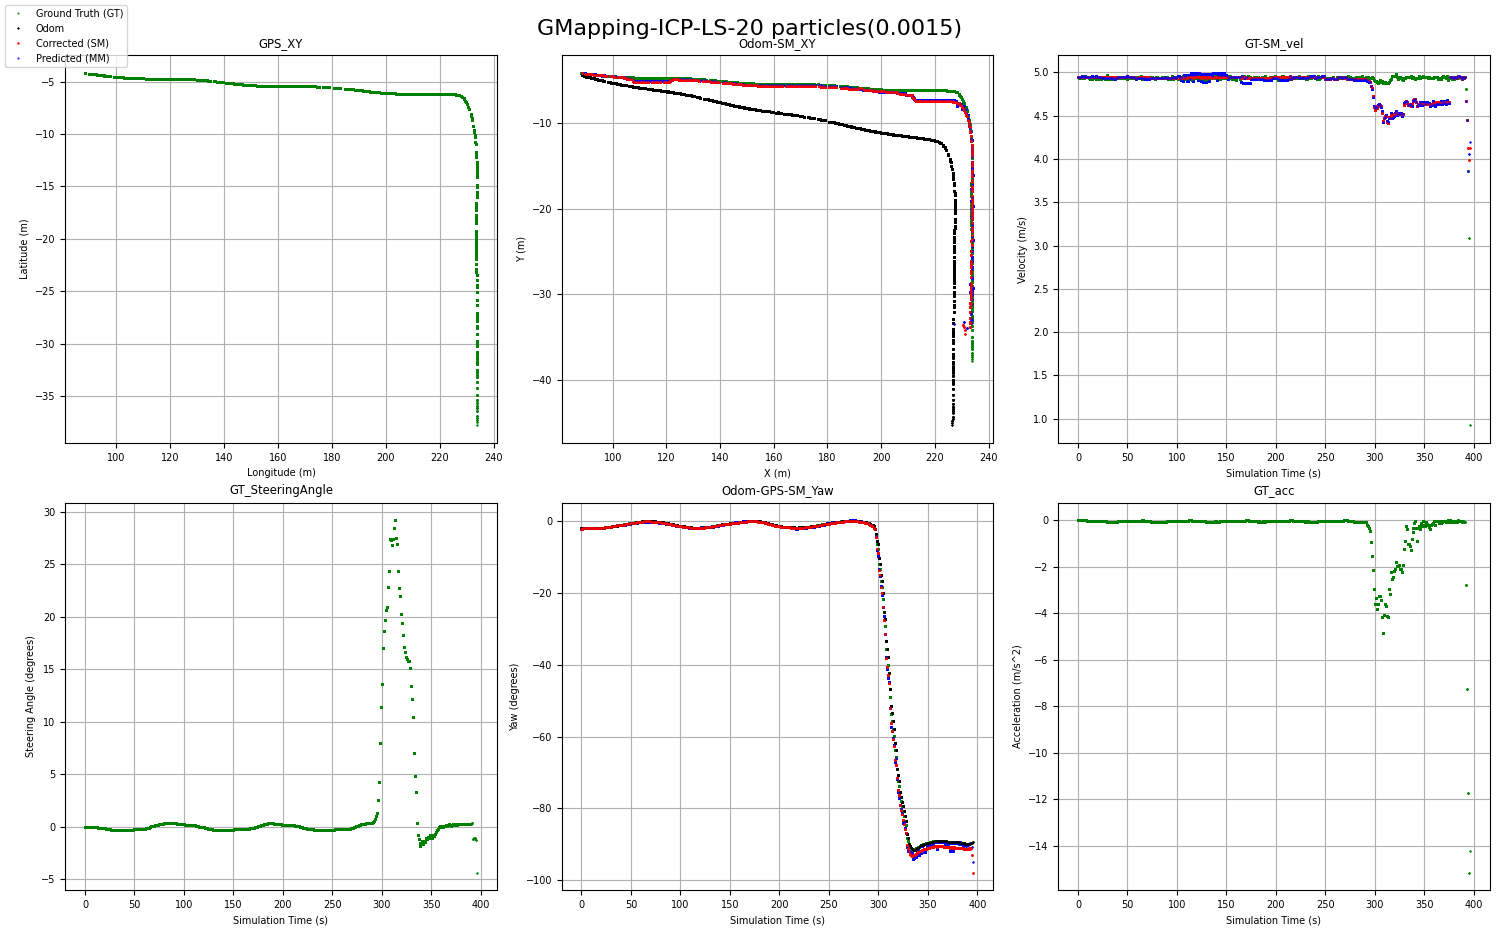
\includegraphics[height=0.6\textwidth]{images/GMapping-ICP-LS-20 particles(0.0015)_PositionParameters.png}
        \caption{LS based ICP- Particles(20), Error Threshold(0.0015). Label:Ground Truth(green), Odometry(black), Motion Model prediction(blue), Scan Matching correction(red)}
        \label{fig:LS_20_0.0025}
    \end{figure}
    \begin{figure}[h] 
        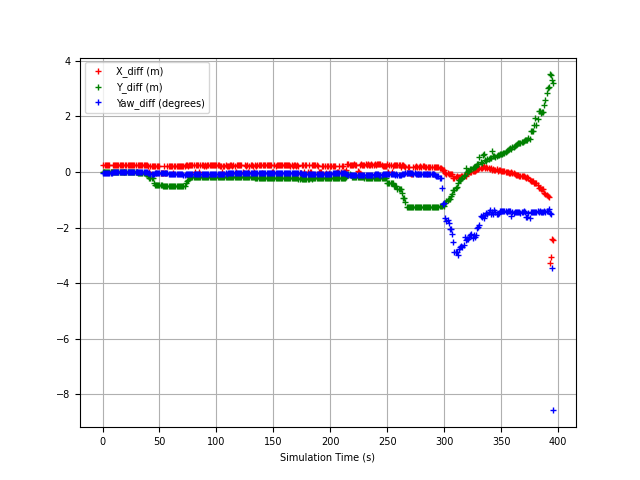
\includegraphics[height=0.4\textwidth]{images/GMapping-ICP-LS-20 particles(0.0015)_True_vs_Crct.png}
        \caption{LS based ICP- Difference between ground truth (GPS) and estimation}
        \label{fig:LS_20_0.0025_diff}
    \end{figure}
\clearpage
Just increasing the number of particles to 50, provides marginally better results than the previous case \ref{fig:LS_50_0.0025}, \ref{fig:LS_50_0.0025_diff}.
    \begin{figure}[h] 
        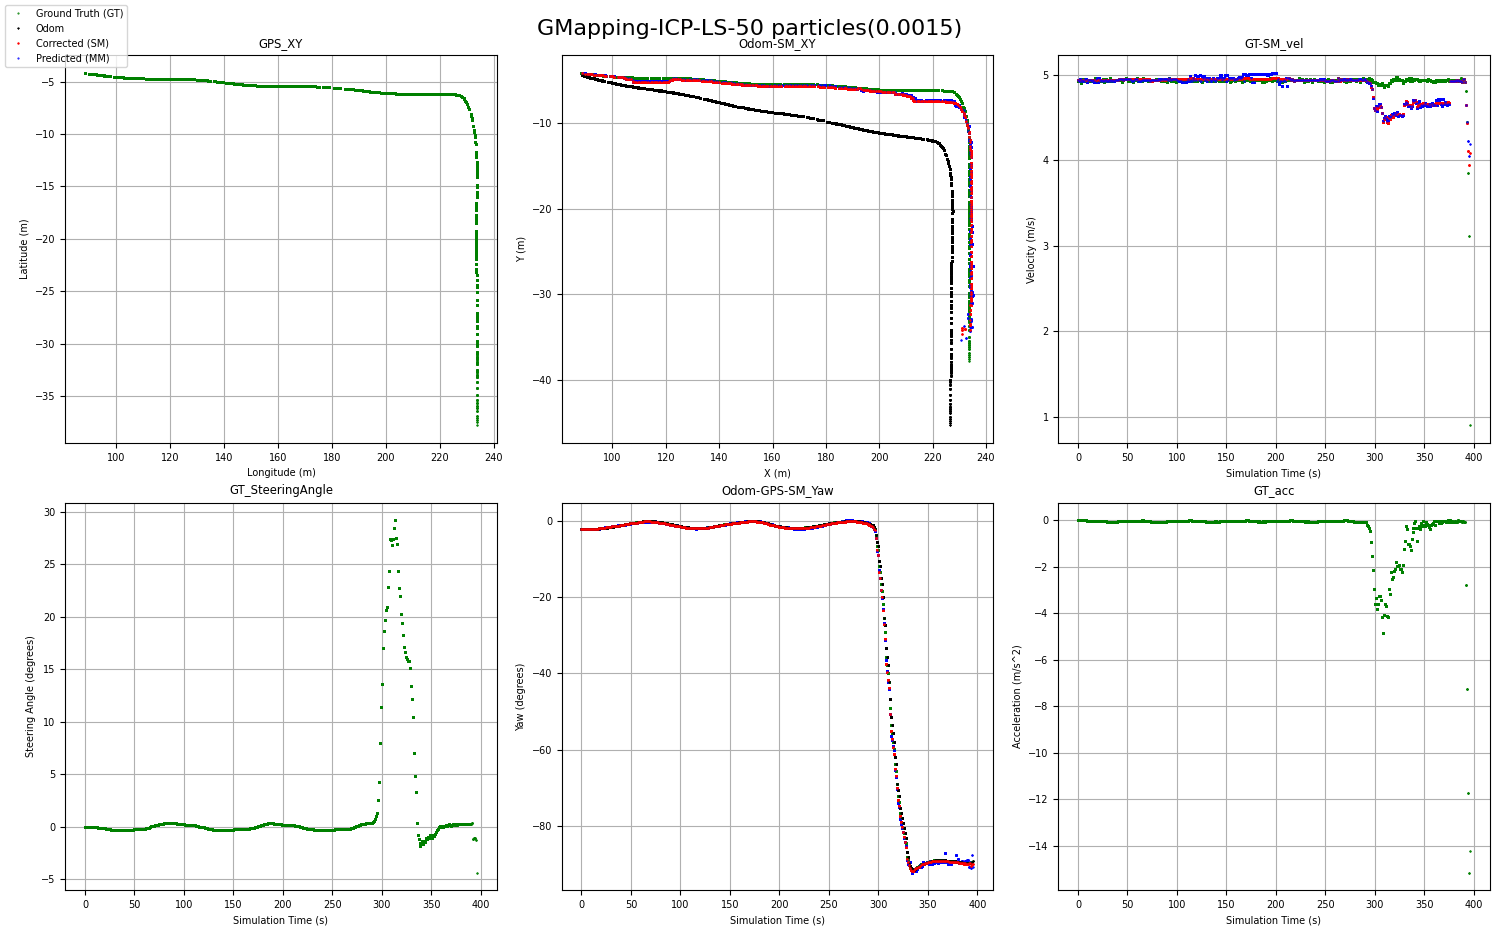
\includegraphics[height=0.6\textwidth]{images/GMapping-ICP-LS-50 particles(0.0015)_PositionParameters.png}
        \caption{LS based ICP- Particles(50), Error Threshold(0.0015). Label:Ground Truth(green), Odometry(black), Motion Model prediction(blue), Scan Matching correction(red)}
        \label{fig:LS_50_0.0025}
    \end{figure}
    \begin{figure}[h] 
        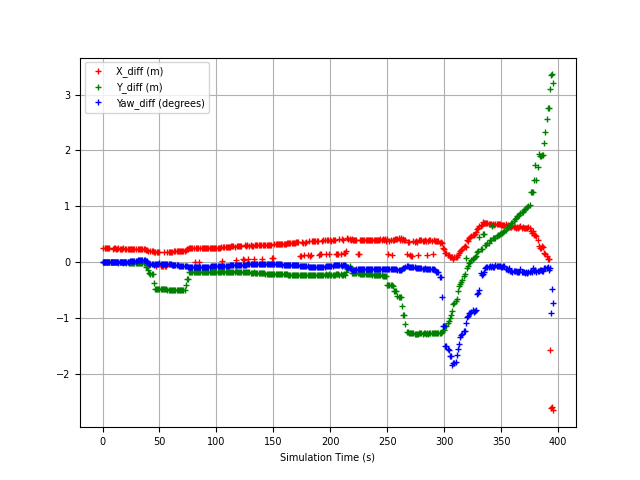
\includegraphics[height=0.4\textwidth]{images/GMapping-ICP-LS-50 particles(0.0015)_True_vs_Crct.png}
        \caption{LS based ICP- Difference between ground truth (GPS) and estimation}
        \label{fig:LS_50_0.0025_diff}
    \end{figure}
\clearpage
However with tighter error threshold(0.001) the performance of the system is better, with pose more aligned to the ground truth \ref{fig:LS_20_0.002}, \ref{fig:LS_20_0.002_diff}.
    \begin{figure}[h] 
        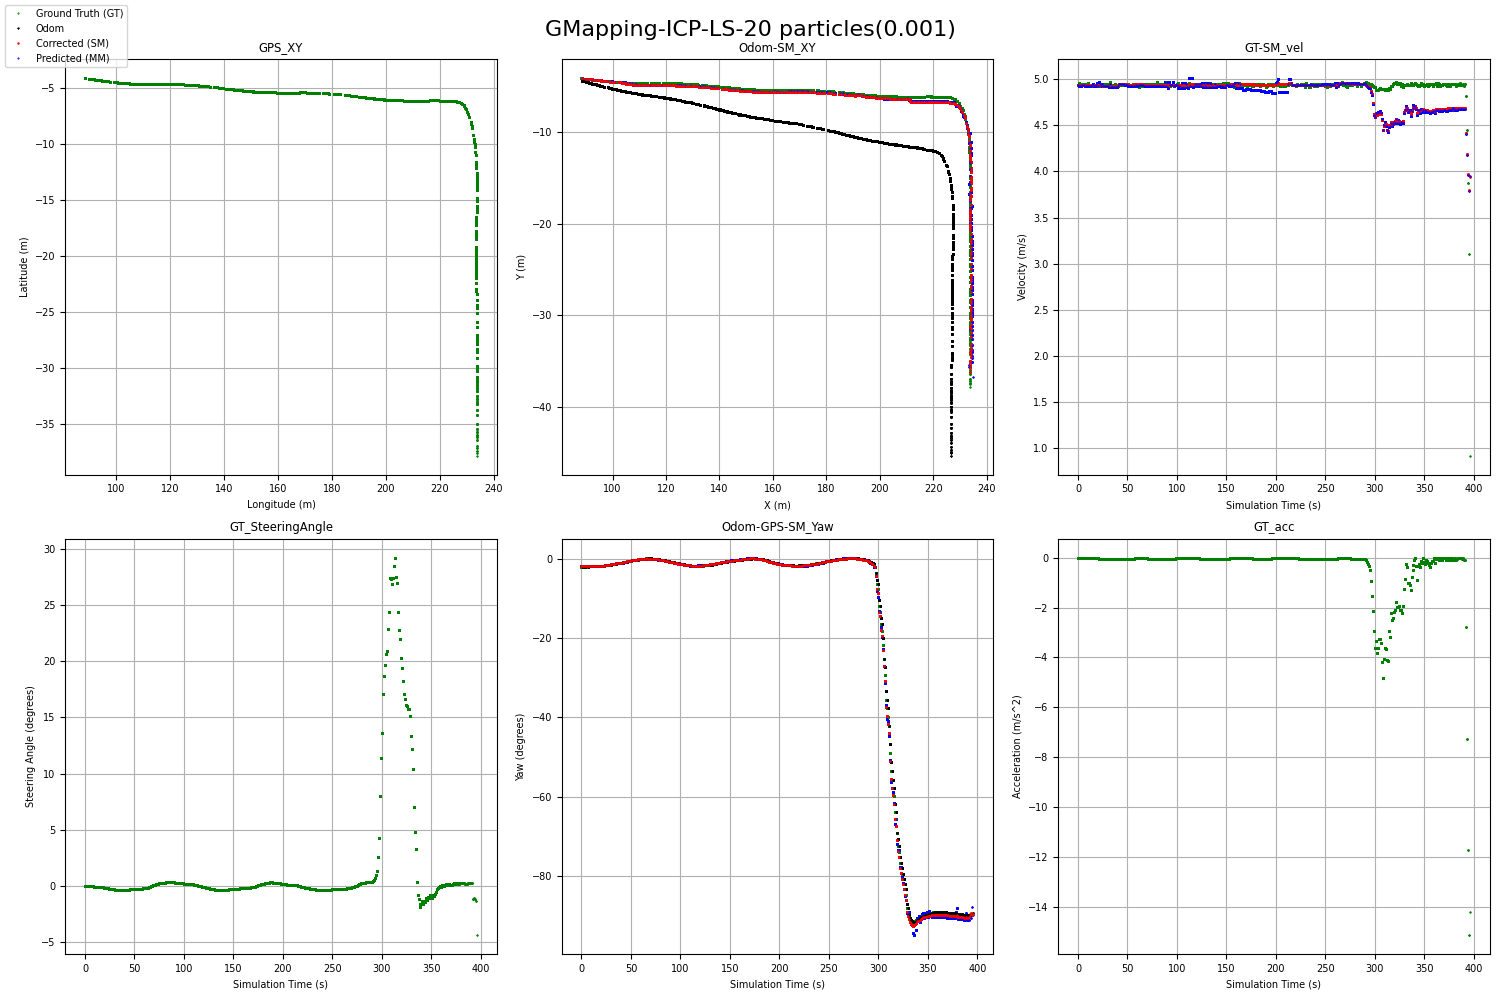
\includegraphics[height=0.6\textwidth]{images/GMapping-ICP-LS-20 particles(0.001)_PositionParameters.png}
        \caption{LS based ICP- Particles(20), Error Threshold(0.001). Label:Ground Truth(green), Odometry(black), Motion Model prediction(blue), Scan Matching correction(red)}
        \label{fig:LS_20_0.002}
    \end{figure}
    \begin{figure}[h] 
        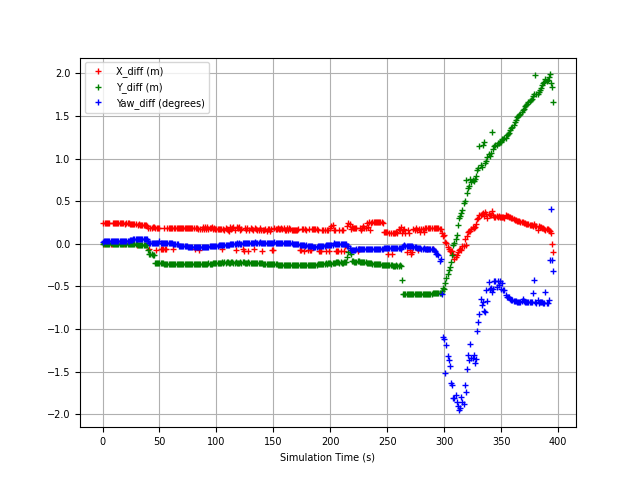
\includegraphics[height=0.4\textwidth]{images/GMapping-ICP-LS-20 particles(0.001)_True_vs_Crct.png}
        \caption{LS based ICP- Difference between ground truth (GPS) and estimation}
        \label{fig:LS_20_0.002_diff}
    \end{figure}
\clearpage
With more number of particles, the results are even better \ref{fig:LS_50_0.002}, \ref{fig:LS_50_0.002_diff}.
    \begin{figure}[h] 
        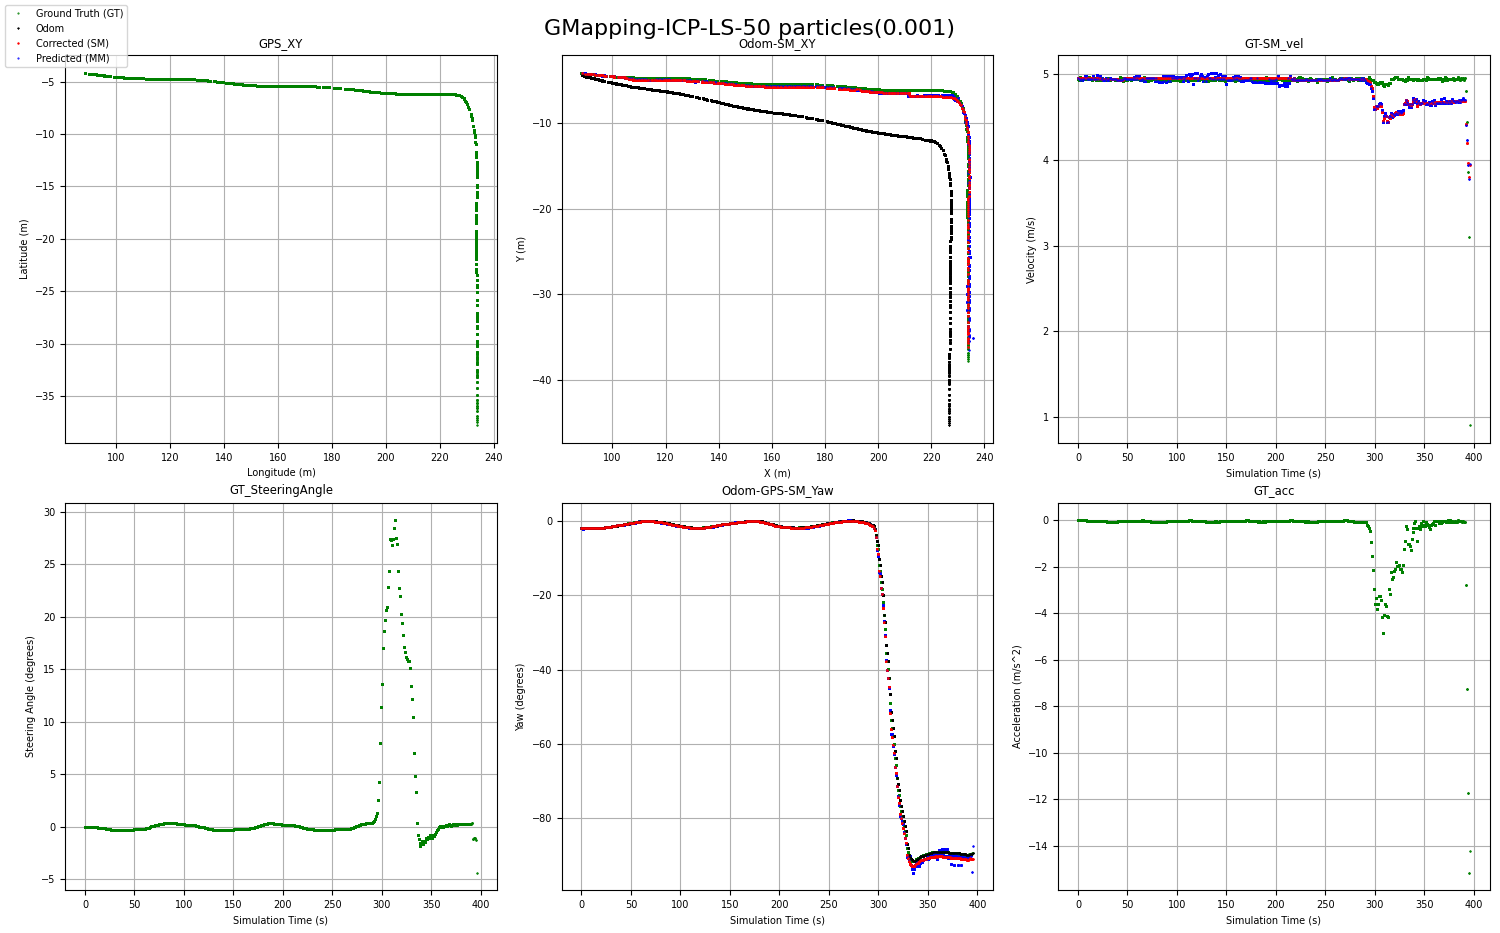
\includegraphics[height=0.6\textwidth]{images/GMapping-ICP-LS-50 particles(0.001)_PositionParameters.png}
        \caption{LS based ICP- Particles(50), Error Threshold(0.001). Label:Ground Truth(green), Odometry(black), Motion Model prediction(blue), Scan Matching correction(red)}
        \label{fig:LS_50_0.002}
    \end{figure}
    \begin{figure}[h] 
        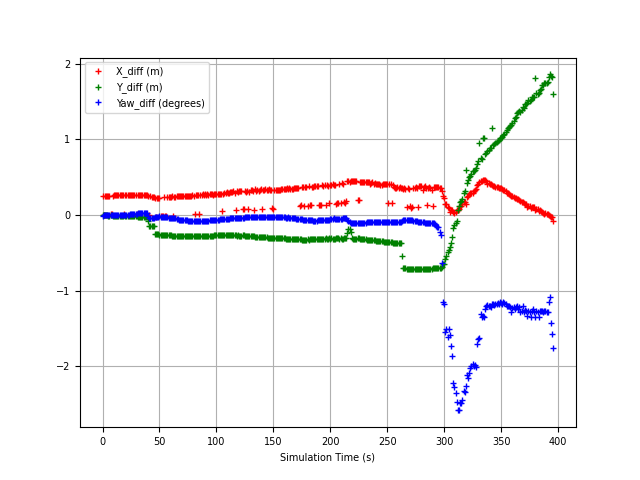
\includegraphics[height=0.4\textwidth]{images/GMapping-ICP-LS-50 particles(0.001)_True_vs_Crct.png}
        \caption{LS based ICP- Difference between ground truth (GPS) and estimation}
        \label{fig:LS_50_0.002_diff}
    \end{figure}
\clearpage

\subsection{Evaluating RTCSM}
Unlike ICP, RTCSM does not have a error threshold but has a confidence to how good the scan matching results are. In the RTCSM algorithm, local map created from the previous pose update is correlated with the local map created from the present particle position. In this process a Gaussian(possible pose estimate as a mask) is placed over every single occupied cell for every possible orientation. The confidence value is calculated that is used as a criteria for acceptance. Similar to ICP, the evaluation is repeated for four possible combinations of particle count (20 and 50) and confidence values (0.052 and 0.05). The increasing difference at the last few seconds in the longitudinal direction is observed in all the following cases because of wrong velocity estimation hence it is not considered in analysis further.
With lower confidence(0.05) and less number of particles(20), a offset can be observed in the pose and orientation estimation \ref{fig:RTCSM_20_0.05}. Like in the case of ICP, It can also be seen that difference in the pose and orientation estimation to the ground truth is never converging \ref{fig:RTCSM_20_0.05_diff}.
    \begin{figure}[h] 
        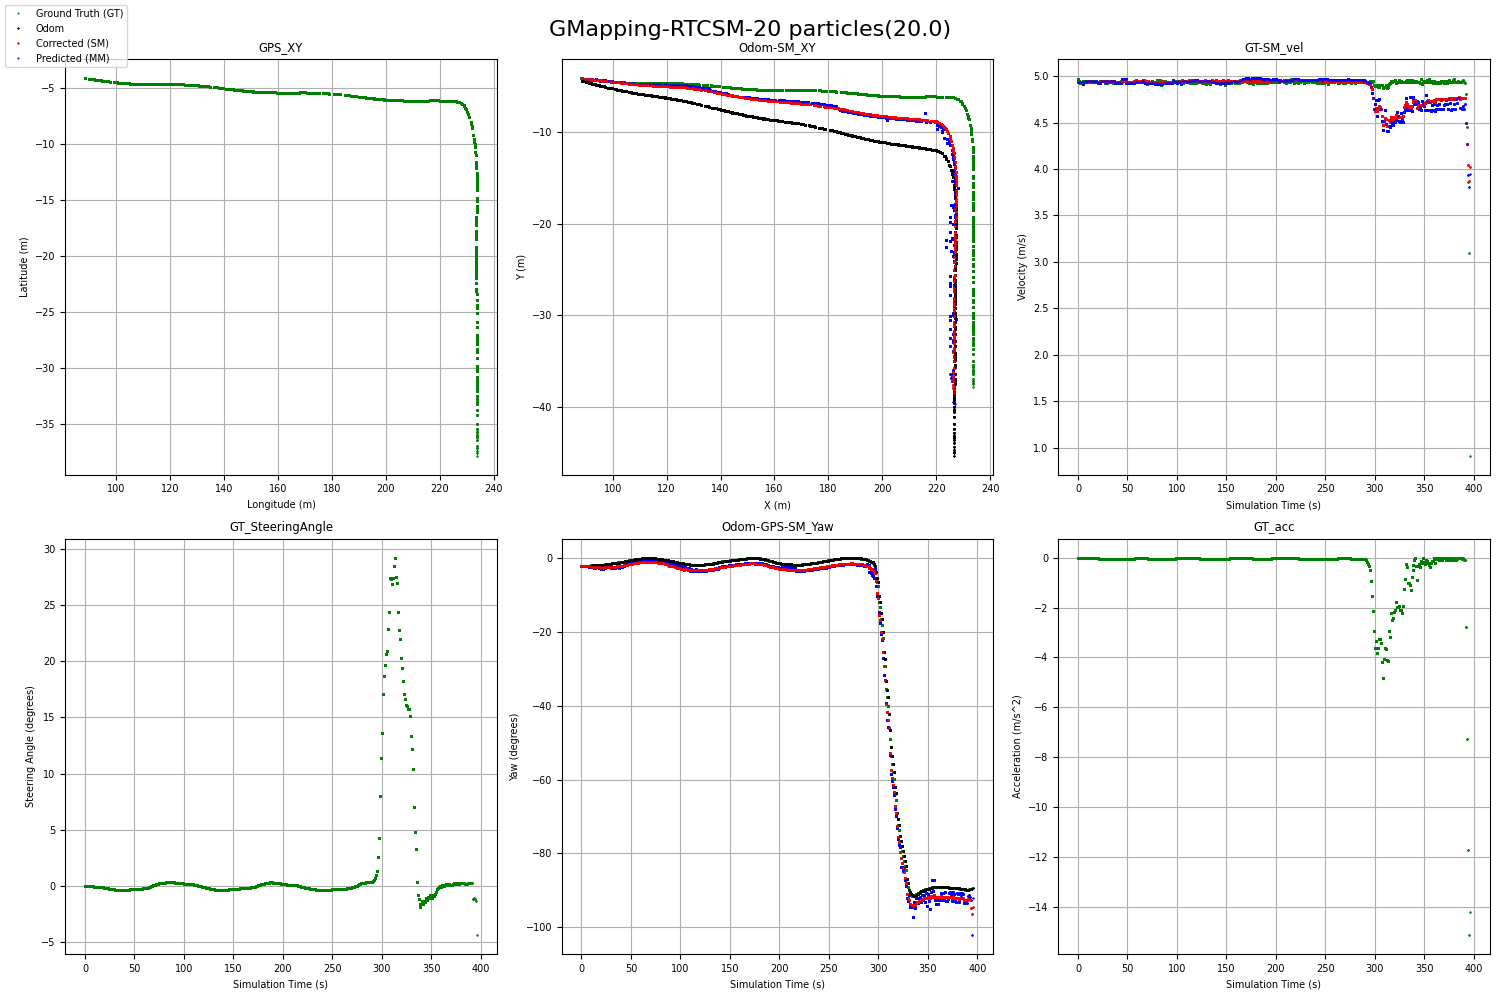
\includegraphics[height=0.6\textwidth]{images/GMapping-RTCSM-20 particles(20.0)_PositionParameters.png}
        \caption{RTCSM- Particles(20), Error Threshold(0.05). Label:Ground Truth(green), Odometry(black), Motion Model prediction(blue), Scan Matching correction(red)}
        \label{fig:RTCSM_20_0.05}
    \end{figure}
    \begin{figure}[h] 
        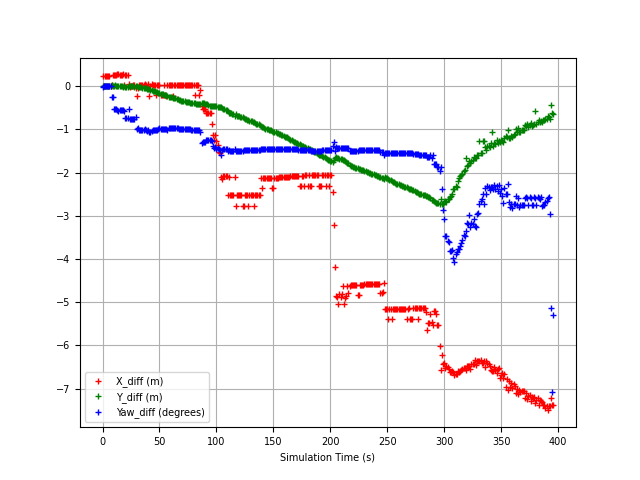
\includegraphics[height=0.4\textwidth]{images/GMapping-RTCSM-20 particles(20.0)_True_vs_Crct.png}
        \caption{RTCSM- Difference between ground truth (GPS) and estimation}
        \label{fig:RTCSM_20_0.05_diff}
    \end{figure}
\clearpage
Just increasing the number of particles to 50, provides marginally better results than the previous case \ref{fig:RTCSM_50_0.05}, \ref{fig:RTCSM_50_0.05_diff}.
    \begin{figure}[h] 
        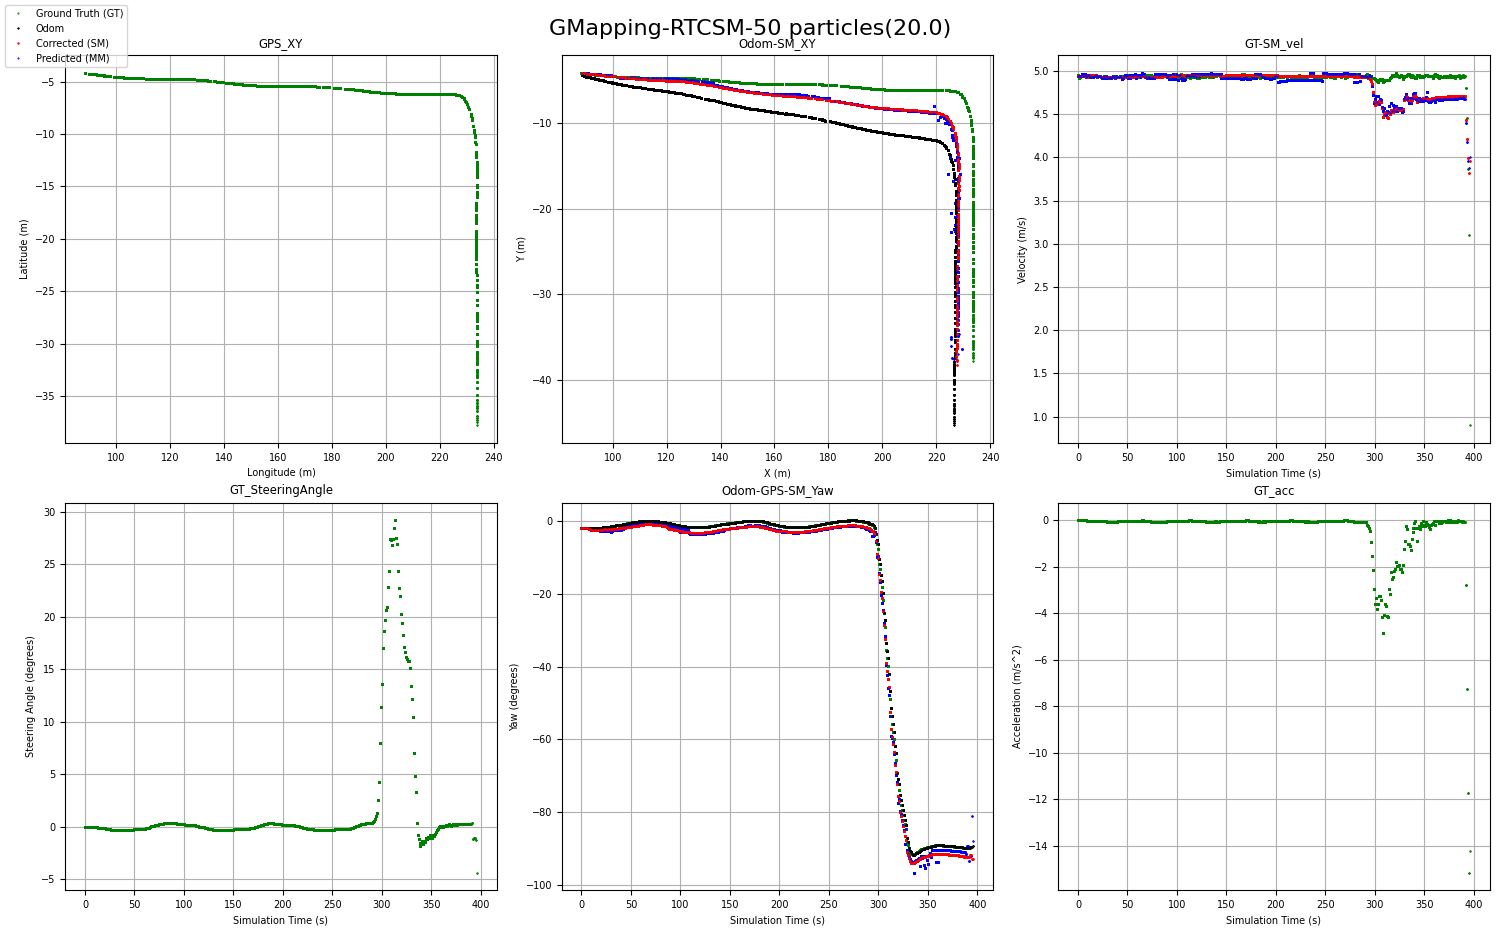
\includegraphics[height=0.6\textwidth]{images/GMapping-RTCSM-50 particles(20.0)_PositionParameters.png}
        \caption{RTCSM- Particles(50), Error Threshold(0.02). Label:Ground Truth(green), Odometry(black), Motion Model prediction(blue), Scan Matching correction(red)}
        \label{fig:RTCSM_50_0.05}
    \end{figure}
    \begin{figure}[h] 
        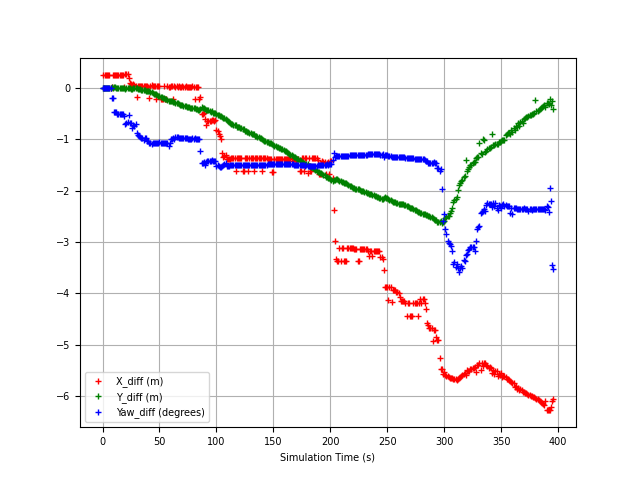
\includegraphics[height=0.4\textwidth]{images/GMapping-RTCSM-50 particles(20.0)_True_vs_Crct.png}
        \caption{RTCSM- Difference between ground truth (GPS) and estimation}
        \label{fig:RTCSM_50_0.05_diff}
    \end{figure}
\clearpage
However with higher confidence threshold(0.052) the performance of the system is better, with pose more aligned to the ground truth \ref{fig:RTCSM_20_0.052}, \ref{fig:RTCSM_20_0.052_diff}.
    \begin{figure}[h] 
        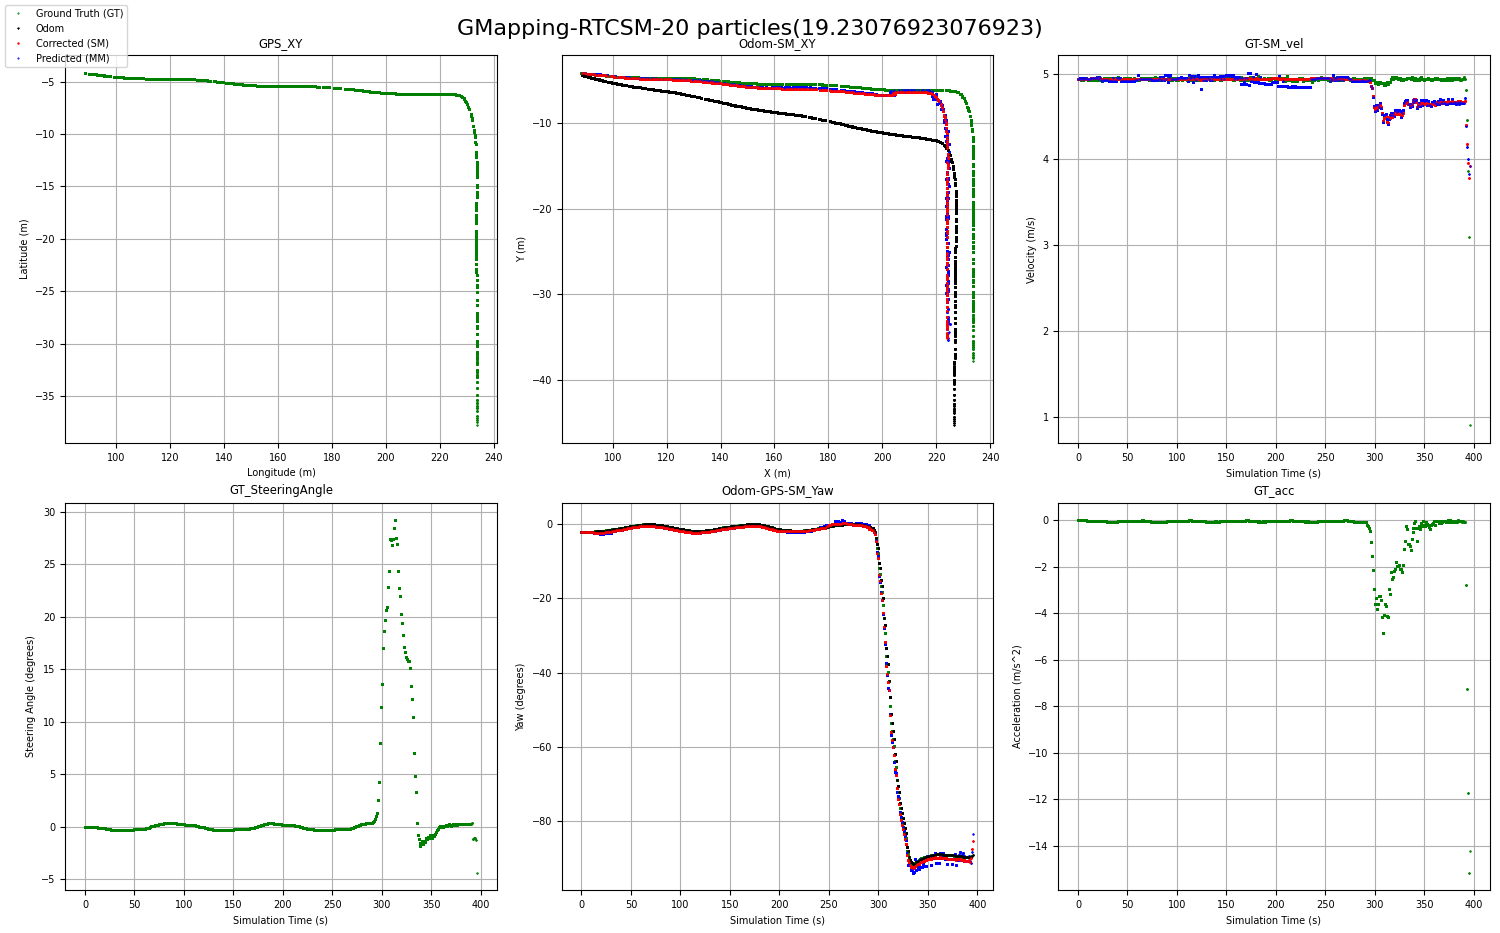
\includegraphics[height=0.6\textwidth]{images/GMapping-RTCSM-20 particles(19.23076923076923)_PositionParameters.png}
        \caption{RTCSM- Particles(20), Error Threshold(0.052). Label:Ground Truth(green), Odometry(black), Motion Model prediction(blue), Scan Matching correction(red)}
        \label{fig:RTCSM_20_0.052}
    \end{figure}
    \begin{figure}[h] 
        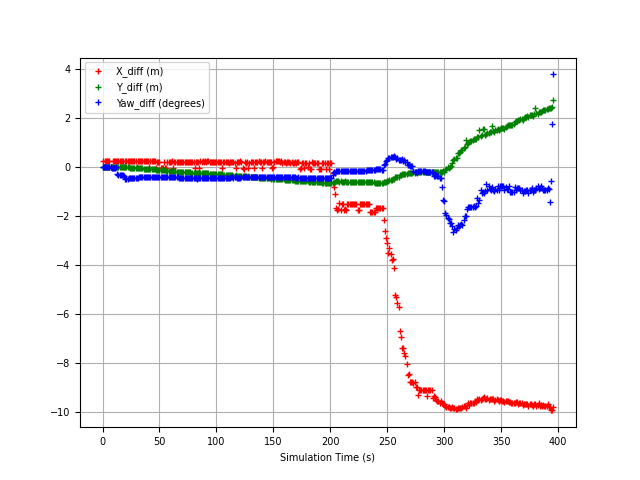
\includegraphics[height=0.4\textwidth]{images/GMapping-RTCSM-20 particles(19.23076923076923)_True_vs_Crct.png}
        \caption{RTCSM- Difference between ground truth (GPS) and estimation}
        \label{fig:RTCSM_20_0.052_diff}
    \end{figure}
\clearpage
With more number of particles, the results are even better \ref{fig:RTCSM_50_0.052}, \ref{fig:RTCSM_50_0.052_diff}.
    \begin{figure}[h] 
        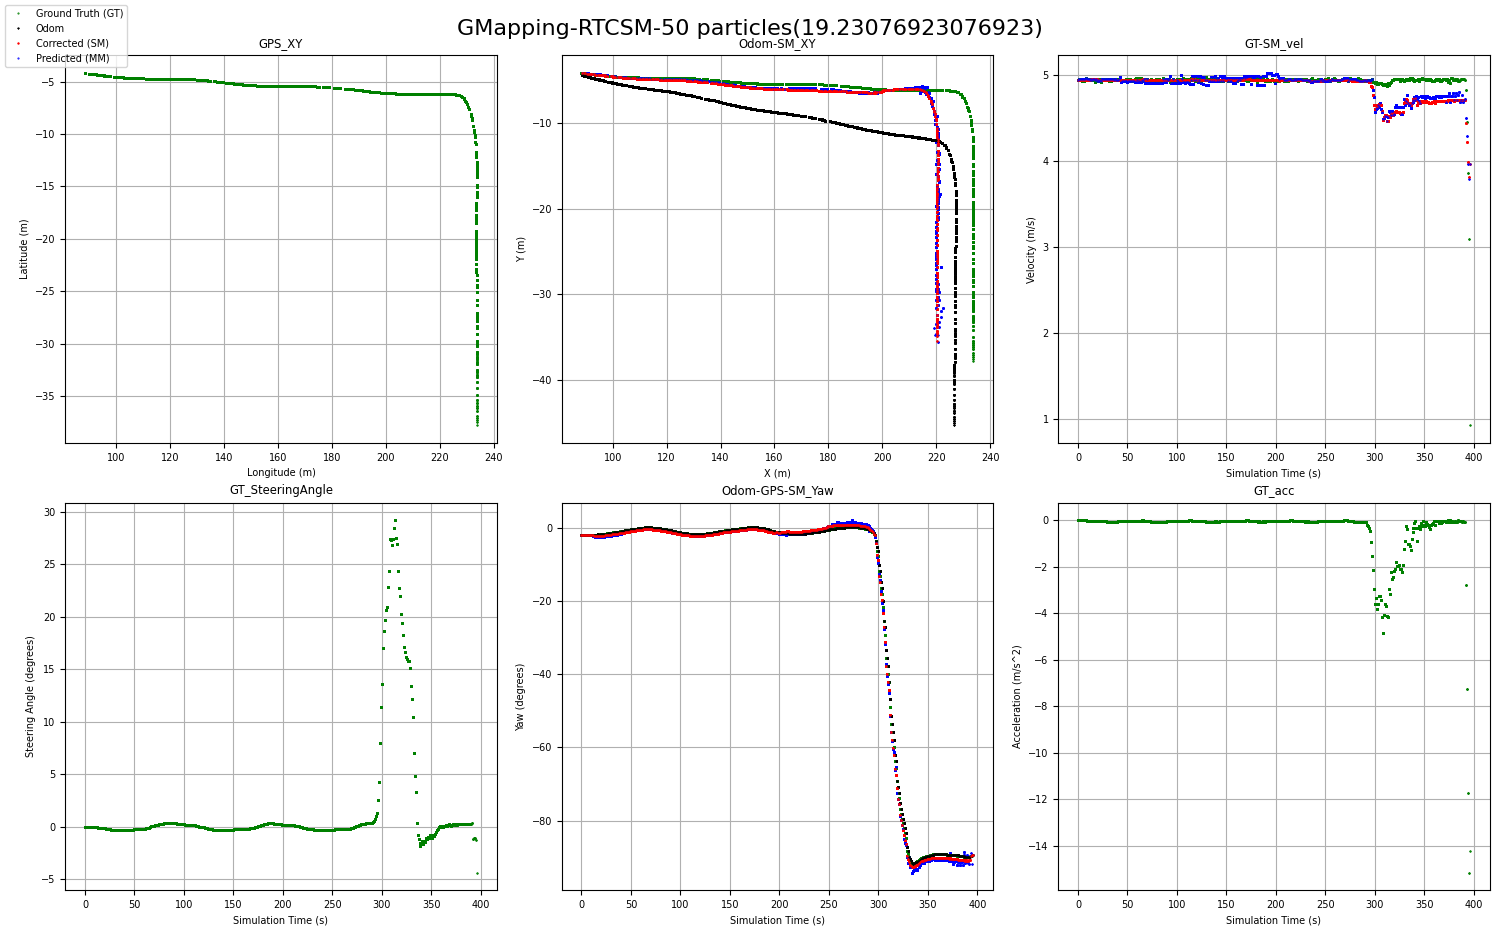
\includegraphics[height=0.6\textwidth]{images/GMapping-RTCSM-50 particles(19.23076923076923)_PositionParameters.png}
        \caption{RTCSM- Particles(50), Error Threshold(0.052). Label:Ground Truth(green), Odometry(black), Motion Model prediction(blue), Scan Matching correction(red)}
        \label{fig:RTCSM_50_0.052}
    \end{figure}
    \begin{figure}[h] 
        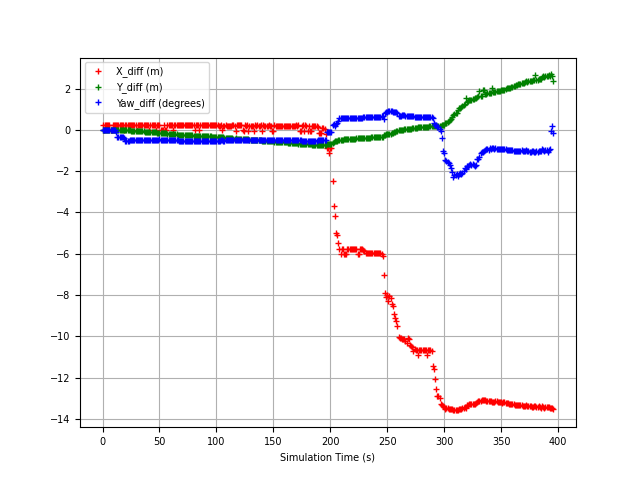
\includegraphics[height=0.4\textwidth]{images/GMapping-RTCSM-50 particles(19.23076923076923)_True_vs_Crct.png}
        \caption{RTCSM- Difference between ground truth (GPS) and estimation}
        \label{fig:RTCSM_50_0.052_diff}
    \end{figure}
\clearpage

\subsection{Overall analysis} \label{ssec:overallanalysis}
The benchmark parameters are calculated and summarised in the figure \ref{fig:benchmark}.
    \begin{figure}[h] 
        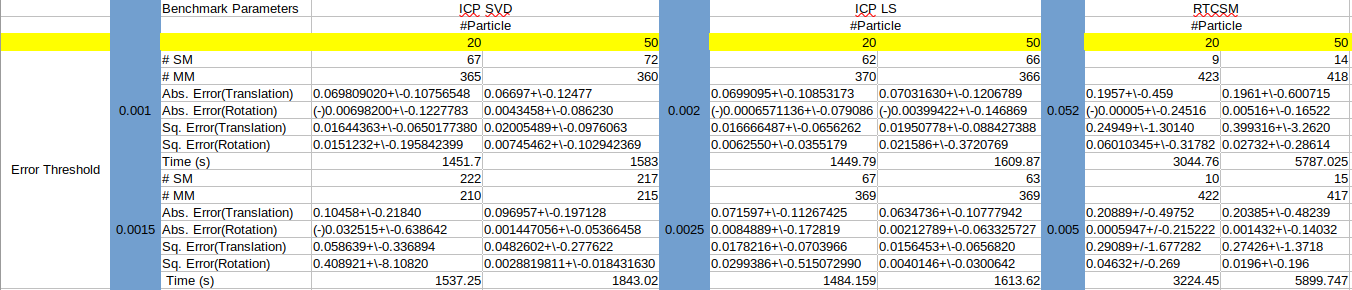
\includegraphics[width=1\textwidth]{images/Benchmark.png}
        \caption{Evaluation result of scan matching algorithms}
        \label{fig:benchmark}
    \end{figure}
In the figure \ref{fig:benchmark}, $#SM$ and $#MM$ denote the number of times scan matching and motion model had been taken into estimation respectively. It can be observed that ICP-LS and ICP-SVD have comparable results in terms of accuracy and computation time with a demanding threshold criteria. However in the case of a relaxed error threshold criteria, ICP-LS performs better. A strict criteria  for the error threshold forces the system to discard the scan matching result for a better map. As an effect the algorithm following it is not executed, resulting in particle states being updated with motion model prediction. 
Both absolute and squared error are considered in the evaluation, they are used widely to evaluate the SLAM algorithms \cite{kuemmerle09auro}. The ICP-LS provides more accurate results than RTCSM or ICP-SVD. Due to implementation difficulties RTCSM could not be run on parallel compute, hence the run time of the algorithm is high. However the accuracy of the algorithm is very low compared to ICP variants

% Conclusions / Findings
\chapter{Conclusions}
The analysis in the previous chapter show that ICP-LS provides better results in terms of accuracy and computation efficiency.The evaluation was only performed over one dataset but could be easily extended  against various datasets.
\par
The study and implementation provide understanding on how efficient are the scan matching algorithms with the current system of particle filter based SLAM. It is also to be noted that the implementation could also be made more efficient with better coding practises or even choice of programming language. The performance could also change cast if the scan matching algorithms are used and evaluated with different approaches of SLAM such as graph based SLAM. This work provides a ground from which many scan matching algorithms can be implemented and evaluated.

% Reflective analysis
\chapter{Reflective Analysis}
\input{chapters/reflective-analysis}





% end of thesis body
% --------------------------

% Print out the references
\printReferences

% Appendices: feel free to comment these out if you are 
% not going to use them.
% Writing appendices is super super easy in LaTeX. You just write
% \appendix to demarcate where the normal content ends and the appendices start. After \appendix, chapters (started with \chapter) are considered as appendices.
%
% In this example though, we're using the appendices environment. Long story short, this is because we want some fancy titles in the toc.
\begin{appendices}

% Appendix A
% ----------

\chapter{Some random python code}
This template includes the \texttt{minted} package, which allows you to import code and syntax highlight it. For example, the text below is imported directly from the \texttt{code/test.py} file using the \textbackslash\texttt{inputminted} command:

\begin{framed}
    \inputminted{python3}{code/test.py}
\end{framed}

And here is a snippet of Python with the \texttt{minted} environment:

\begin{framed}
\begin{minted}[breaklines]{python}
# Why don't you try running this?
# See what it does? hm?

m = [ 2, 3, 0, 1, 4 ];
x = [ 'rmdq', 'd', 'n`slk', 'odftp`v)', 'hdk' ];

c = ''.join(list(map(lambda y: chr(ord(y) ^ 5).upper() + ' ' if y != ' ' else '  ', ' '.join([ x[m[i]] for i, v in enumerate(x) ]))));

print('%s\r\n%s\r\n%s\r\n' % ('=' * len(c), c, '=' * len(c)));
\end{minted}
\end{framed}

\cleardoublepage
Minted supports many, many languages -- so you're not just limited to Python. For example, here's some random C++ code.

\begin{framed}
\begin{minted}[breaklines]{cpp}
void CTimesTable::Print(const int number, const int upTo) const
{
    for(int i = 1; i <= upTo; i++)
        printf("%d x %d = %d\r\n", number, i, number * i);
}
\end{minted}
\end{framed}







% Appendix B
% ----------

\chapter{Some other stuff}
Here is just an example of some other stuff.

% End of appendices
\end{appendices}


\end{document}
